\chapter{Data and MC preparation for the Cross Section Measurements}\label{ch:samples}
{\raggedleft ``\emph{Il dolce non lo mangi mai, ma qualche volta ti rifai.} \par}
{\raggedleft \emph{Abbracciami}"\par}
{\raggedleft -- Pietro Ciampi, L'amore e' tutto qui, 1971 -- \par}
\vspace{0.5cm}



This chapter describes the  work done on the  data and Monte Carlo samples in preparation for the cross section analyses. 
This entails the choice of the datasets and the production of the information needed to construct the Monte Carlo Simulation~(Section  \ref{sec:dataSet}),  the construction and use of said Monte Carlo simulation~(section \ref{sec:MCSet}), the study of backgrounds for the pion cross section~(Section  \ref{ch:PionXSBkgSub}), the study of the energy loss between WC4 and TPC (Section \ref{ch:eloss}), the study of the tracking in the TPC~(Section  \ref{sec:TrackingStudies}), and study of  the calorimetry response ~(Section  \ref{ch:energyCal}). 


\section{Cross Section Analyses Data Sets}\label{sec:dataSet}
We choose LArIAT Run-II as the data period for the  ($\pi^{-}$,Ar) and (K$^{+}$,Ar) total hadronic cross section analyses. 
Data taking for the this period started on 03/15/2016  and ended on 07/31/2016. 
Since we are interested in beamline and TPC information, we ask basic requirements on the operational status of the time of fight, wire chambers and TPC to form the good run list for this period, which we informally call ``lovely runs".

The subset of lovely runs  chosen for the  ($\pi^{-}$,Ar) total hadronic cross section analysis includes only the -60A and -100A magnet configurations in negative polarity, even if LArIAT explored several other beamline configurations during Run-II. The -60A and -100A combined data set accounts for approximately 90\% of the total Run-II negative polarity runs.   The  choice of the main two beamline settings limits the need for the production of many different MC sets and related corrections, still maintaining a high number of events. 
%Since the production of beamline Monte Carlo depends on the wanted beamline configuration, the choice of only two beamline settings limits the need for beamline MC production. 

Similarly, the subset of lovely runs chosen  for the (K$^{+}$,Ar)  total hadronic cross section analysis includes only the +60A and +100A magnet configurations in positive polarity. It should be noted that kaons are extremely rare in the +60A sample, thus the data sample for the (K$^{+}$,Ar) cross section after the mass selection is about 90\% +100A runs, as shown in Table \ref{tab:databreakdown}.

For the first measurements in LArIAT that uses both beamline and TPC information, we choose strict requirements on the reconstruction of the WC tracks, the so-called ``Picky Track" sample (see Section \ref{sec:MWPCfunc}). This choice presents two advantages:  the uncertainty on the momentum reconstruction for the ``Picky Tracks" sample is smaller compared to the ``High Yield" sample, and the comparison with the beamline MC results is straightforward. A possible future update and cross check of these analysis would be the use of the High Yield sample, where the statistics is about three times higher. 

The breakdown of beamline events as a function of the magnets settings is shown in Table \ref{tab:databreakdown}. 
The choice of the data sets determines the production of beamline MC and serves as basis for the production of Data Driven MC, as shown in the next sections.

\begin{table}[b]
\centering
\begin{tabular}{|l|c|c|c|}  
\hline
                                                              & I = 60 A          & I = 100 A   & Total     \\ \hline
Data Events after $\pi/\mu/e$ Mass Selection     &     67068          &  71413  & 138481 \\ \hline
Data Events after $K$ Mass Selection                &     274              &   2563   & 2837  \\ \hline
\end{tabular}
\caption{Number of data events which fit the $\pi/\mu/e$ or $K$ mass hypothesis as a function of magnet settings.}
\label{tab:databreakdown}
\end{table}



\section{Construction of a Monte Carlo Simulation for LArIAT}\label{sec:MCSet}
For the simulation of LArIAT events and for the simulation of the datasets' particle make up, we use a combination of two MC generators: the G4Beamline Monte Carlo and the Data Driven single particle Monte Carlo (DDMC). We use the G4Beamline MC to simulate the particle transportation in the beamline and calculate the particle composition of the beam just after the fourth Wire Chamber (WC4). In order to simulate the beamline particles after WC4 and in the TPC, we use the DDMC.

\subsection{G4Beamline}\label{ch:beamlineComposition}
G4Beamline simulates the beam collision with the LArIAT secondary target, the energy deposited by the particles in the LArIAT beamline detectors, and the action of the LArIAT magnets, effectively accounting for particle transportation through the beamline from the LArIAT target until ``Big Disk", a fictional, void detector located just before the LArIAT cryostat. 
 At the moment of this writing, G4Beamline does not simulated the responses of the beamline detectors. It is possible to interrogate the truth level information of the simulated particles in several points of the geometry. In order to ease the handshake between G4Beamline and the DDMC, we ask for the beam composition just after WC4.
Since LArIAT data are taken under different beam conditions, we need to simulate separately the beam composition according to the magnets' settings and the secondary beam intensity with G4Beamline. For the pion cross section analysis the relevant beam conditions are  secondary beam energy of 64 GeV, negative polarity magnet with current of 100 A and 60 A. For the kaon cross section analysis the relevant beam conditions is a secondary beam energy of 64 GeV, positive polarity magnet with current of 100 A. 

\subsubsection{Beam Composition for Negative Pion Cross Section}
Even if pions are by far the biggest beam component in negative polarity runs, the LArIAT tertiary beam is not a pure pion beam. While useful to discriminate between pions, kaons, and protons, the beamline detectors are not sensitive enough to  discriminate among the lighter particles in the beam: electrons, muons and pions fall under the same mass hypothesis. Thus, we need to assess the contamination from beamline particles other than pions in the event selections used for the pion cross section analysis and correct for its effects. The first step of this process is assessing the percentage of electrons and muons in the $\pi/\mu/e$ beamline candidates via the G4Beamline MC. 
Since the beamline composition is a function of the magnet settings, we simulate separately events for magnet current of -60A and -100A. 
Figure \ref{fig:BeamComposition} shows the momentum predictions from G4Beamline overlaid with data for the 60A runs (left) and for the 100A runs (right). The predictions for electrons, muons and pions have been staggered and their sum is area normalized to data. Albeit not perfect, these plots show a reasonable agreement between the momentum shapes in data and MC.  We attribute the difference in shape to a two approximations performed in the MC. Firstly, G4Beamline lacks the simulation of the WC efficiency which is momentum dependent and leads to enhance the number events in the center of the momentum distribution. Secondly, G4Beamline stop tracking pions and their products if they decay in after WC1; in data, pion decays in flight can still create a tigger if the produced muon travels thought the beamline detectors. In the pion cross section analysis, these differences between data and G4Beamline are accounted for as a systematic uncertainty related to the beam composition (see Section \ref{ch:BKGsubXSPuppa}).
%We attribute  the difference in shape to the lack of simulation of the WC efficiency in the MC which is momentum dependent and leads to enhance the number events in the center of the momentum distribution.


\begin{figure}
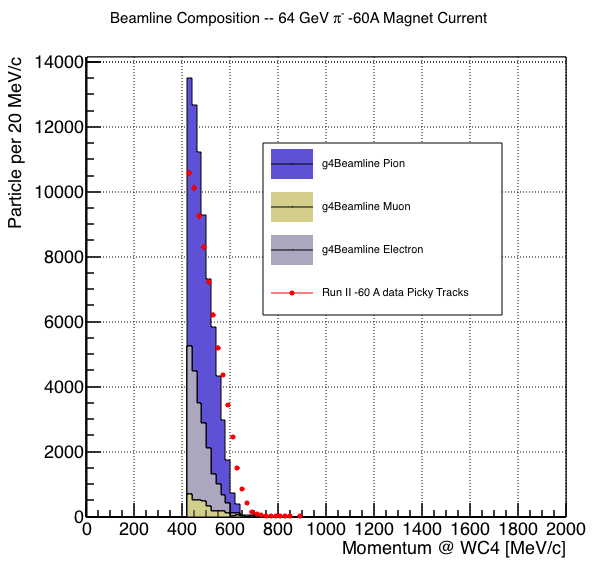
\includegraphics[width=0.5\textwidth,height=\textheight,keepaspectratio]{Chapter-5/Images/Beam60A.png}
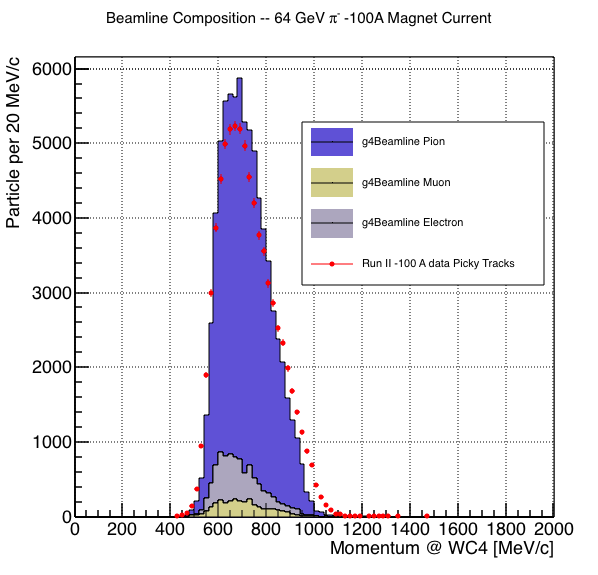
\includegraphics[width=0.5\textwidth,height=\textheight,keepaspectratio]{Chapter-5/Images/Beam100A.png}
\caption{Beam composition for the -60A runs (left) and -100A runs (right). The solid blue plot represents the simulated pion content, the yellow plot represents the simulated muon content and the grey plot represents the simulated electron content. The plots are area normalized to the number of data events, shown in red. }
\label{fig:BeamComposition}
\end{figure}

Table \ref{tab:beamline} shows the beam composition per magnet setting after the mass selection according to the G4Beamline simulation.
\begin{table}[]
\centering
\begin{tabular}{|l|c|c|}
\hline
                     & I = -60 A           & I = -100 A \\ \hline
G4Pions       &   68.8 \%           &      87.4 \%        \\ \hline
G4Muons     &     4.6 \%           &        3.7 \%         \\ \hline
G4Electrons &   26.6 \%           &        8.9 \%        \\ \hline
\end{tabular}
\caption{Simulated beamline composition per magnet settings}
\label{tab:beamline}
\end{table}

The estimated beam composition is used as a basis to estimate the background contamination in the  ($\pi^{-}$,Ar) cross section measurement, whose  full treatment is described in section \ref{ch:PionXSBkgSub}.

\subsubsection{Beam Composition for Positive Kaon Cross Section}
In the positive polarity runs, the tertiary beam composition is mainly pions and protons. The left side of Figure \ref{fig:BeamCompositionPos} shows the  predictions for the momentum spectra for the 100A positive runs  according to  G4Beamline (solid colors) overlaid with data (black points). 
Since the LArIAT beamline detectors can discriminate between kaons and other particles, we do not rely on the G4Beamline simulation to estimate the beamline contamination in the pool of kaon candidates (as in the case of the pion cross section), but rather we use a data drive approach. 
The basic idea of this data driven approach is to estimate the bleed over from high and low mass peaks under the kaon peak by fitting the tails of the $\pi/\mu/e$ and proton mass distributions, as shown in Figure \ref{fig:BeamCompositionPos} right side. 
Since the shape of the tails is unknown, the estimate is done multiple times varying the range and shape for reasonable functions. 
For example, to estimate the proton content under the kaon peak, we start by fitting the left tail of the proton mass distribution with a gaussian function between 650 $MeV/c^2$ and 750 MeV/c$^2$. % in a reasonable range and with a reasonable function. 
 We extend the fit function under the kaon peak and integrate the extended fit function between 350-650 MeV/c$^2$. We integrate the mass histogram in the same range and calculate the proton contamination as the ratio between the two integrals. We repeat this procedure for several fit shapes (gaussian, linear and exponential functions) and tail ranges. Finally, we calculate the contamination as the weighted average of single estimates, where the weights are calculated to be the $1./|1-\chi^2|$ of the tail fits. The procedure is repeated for lighter particles mass peak independently.
With 12 iterations of this method we find a proton contamination of  5.0 $\pm$ 2.0 \%  and a contamination from the lighter particles of 0.2 $\pm$ 0.5 \% .
The estimate of the proton background is currently not used in the kaon cross section analysis, but it is a fundamental step to retrieve the true kaon cross section which will be implemented in the further development of the analysis.


\begin{figure}
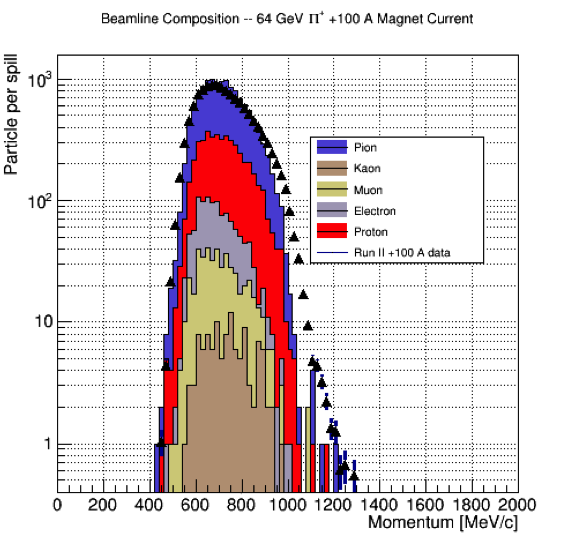
\includegraphics[width=0.5\textwidth,height=\textheight,keepaspectratio]{Chapter-5/Images/Beam100Pos.png}
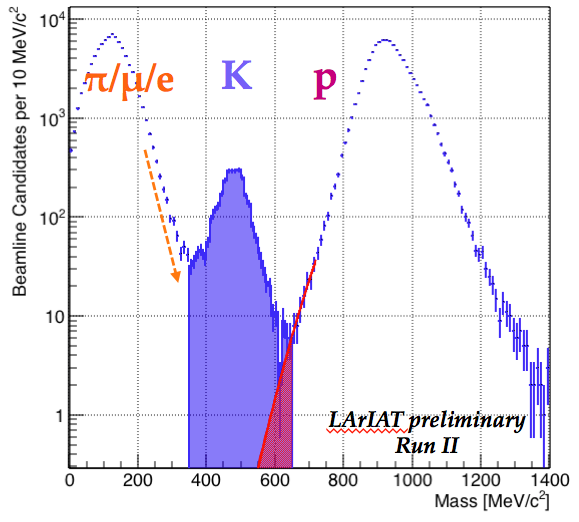
\includegraphics[width=0.5\textwidth,height=\textheight,keepaspectratio]{Chapter-5/Images/MassPos.png}
\caption{\emph{Left:} Beam composition for the +100A runs after WC4 (no mass selection applied). The solid colors represent the contributions from the G4Beamline simulated particles: blue plot represents the simulated pion content, the yellow plot represents the simulated muon content and the grey plot represents the simulated positron content, the red the proton content and the mustard the kaon content. The plots are area normalized to the number of data events, shown in black. \emph{Right:} Mass distribution for the Run-II positive runs, where the area under the kaon mass peak is highlighted in purple. The area under the extension of a possible fit for the proton tail is highlighted in red. }
\label{fig:BeamCompositionPos}
\end{figure}



\subsection{Data Driven MC}\label{sec:DDMC}
The Data Driven single particle Monte Carlo (DDMC) is a single particle gun which simulates the particle transportation from WC4 into the TPC leveraging on the beamline data information. The DDMC uses the data momentum and position at WC4 to derive the event generation: a general sketch of the DDMC workflow is shown in Figure \ref{fig:DDMCSketch}.

When producing a DDMC sample, beamline data from a particular running period and/or running condition are selected first. For example, data for the negative 60A runs and for the negative 100A runs inform the event generation stage of two different DDMC samples. Figure \ref{fig:DDMCQuantities}  schematically shows the data quantities of interest leveraged from data: the momentum ($P_x, P_y, P_z$) and position ($X, Y$) at WC4. For each data event, we obtain the  particle position ($X, Y$) at WC4 directly from the data measurement; we calculate the components of the momentum using the beamline measurement of the momentum magnitude in conjunction with the hits on WC3 and WC4 to determine the direction of the momentum vector, as described in section \ref{sec:MWPCfunc}. The momentum and position of the selected data form a 5-dimensional tupla, which we sample thousands of times through a 5-dimensional hit-or-miss sampling procedure to generate the MC events. This sampling generates MC events  with the same momentum and position distributions as data, with the additional benefit of accounting for the correlations between the $P_x, P_y, P_z, X, Y$ variables.  As an example, the results of the DDMC generation compared to data for the kaon +100A sample are shown in figure \ref{fig:DDMCComparison} for the $P_z$, $X$ and $Y$ distributions; as expected, MC and data agree within the statistical uncertainty by construction. A LArSoft simulation module then launches single particle MC from z = -100 cm (the location of the WC4) using the generated events. The particles are free to decay and interact in their path from WC4 to the TPC according to the Geant4 simulation.

Using the DDMC technique ensures that the MC and data particles have very similar momentum, position and angular distributions at WC4 and allows us to use the MC sample in several occasions: to estimate the background contamination to the pion cross section (see Section \ref{ch:PionXSBkgSub}), to calibrate the energy loss upstream of the TPC (see Section \ref{ch:eloss}),  or to study the tracking and the calorimetric performance (sections \ref{sec:TrackingStudies} and \ref{ch:energyCal}). A small caveat is in order here: the DDMC is a single particle Monte Carlo, which means that the beam pile-up is not simulated. 


We generate six samples for the pion cross section measurement: three samples of  $\sim$330000 pions, muons and electrons to simulate the negative 60A runs, and three samples of $\sim$340000 pions, muons and electrons for the negative 100A runs. We generate a sample of  195000  kaons for the kaon cross section analysis.

\begin{figure}[hpbt]
\centering
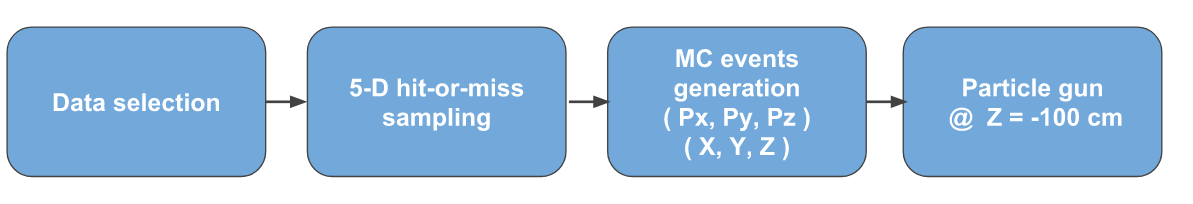
\includegraphics[width=\textwidth]{Chapter-5/Images/DDMCScheme.png}
\caption{Workflow for Data Driven single particle Monte Carlo production.}
\label{fig:DDMCSketch}
\end{figure}


\begin{figure}[hpbt]
\centering
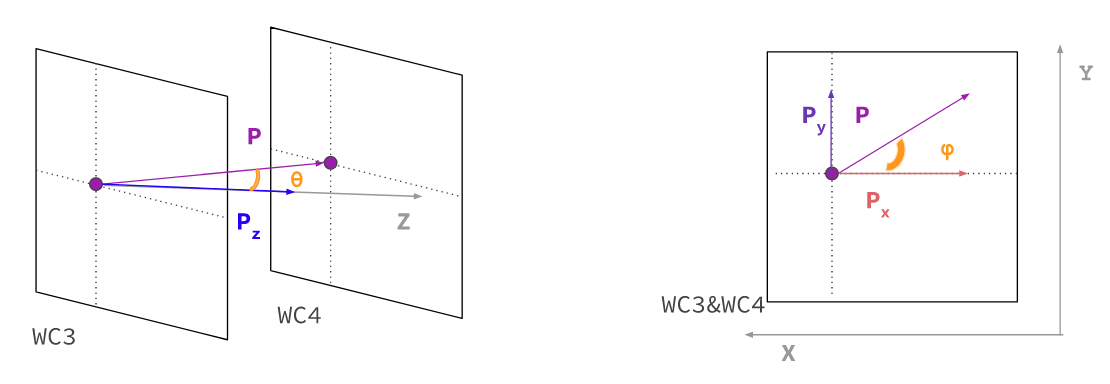
\includegraphics[width=\textwidth]{Chapter-5/Images/DDMCQuantities.png}
\caption{Scheme of the quantities of interest for the DDMC event generation: $P_x, P_y, P_z, X, Y$ at WC4.}
\label{fig:DDMCQuantities}
\end{figure}


\begin{figure}[hpbt]
\centering
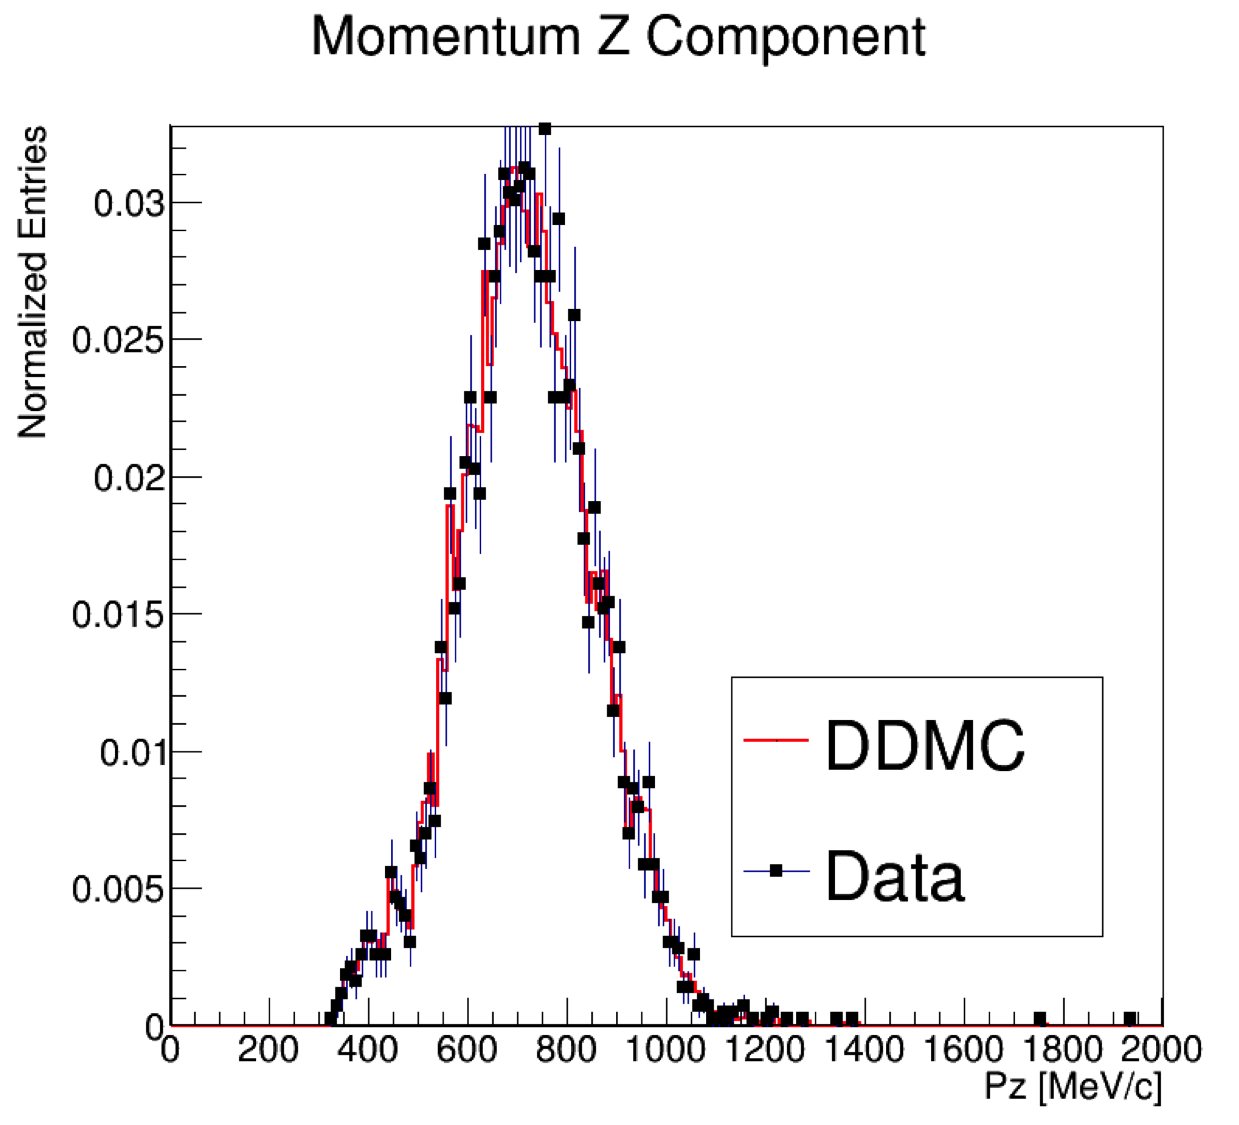
\includegraphics[width=0.48\textwidth]{Chapter-5/Images/DDMCPz.png}
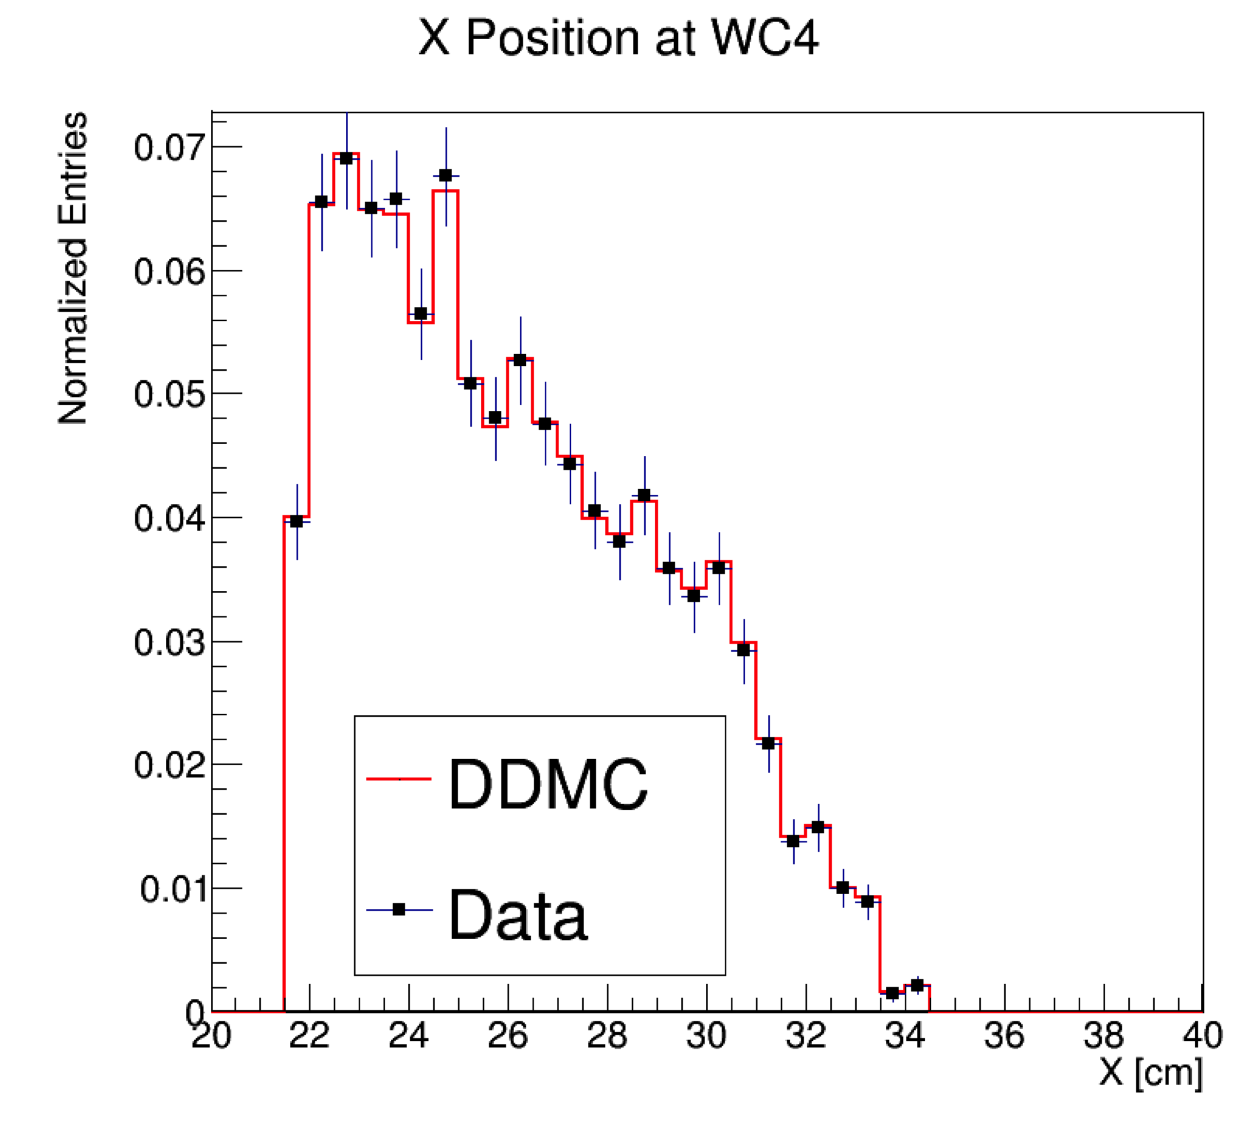
\includegraphics[width=0.48\textwidth]{Chapter-5/Images/DDMCX.png}
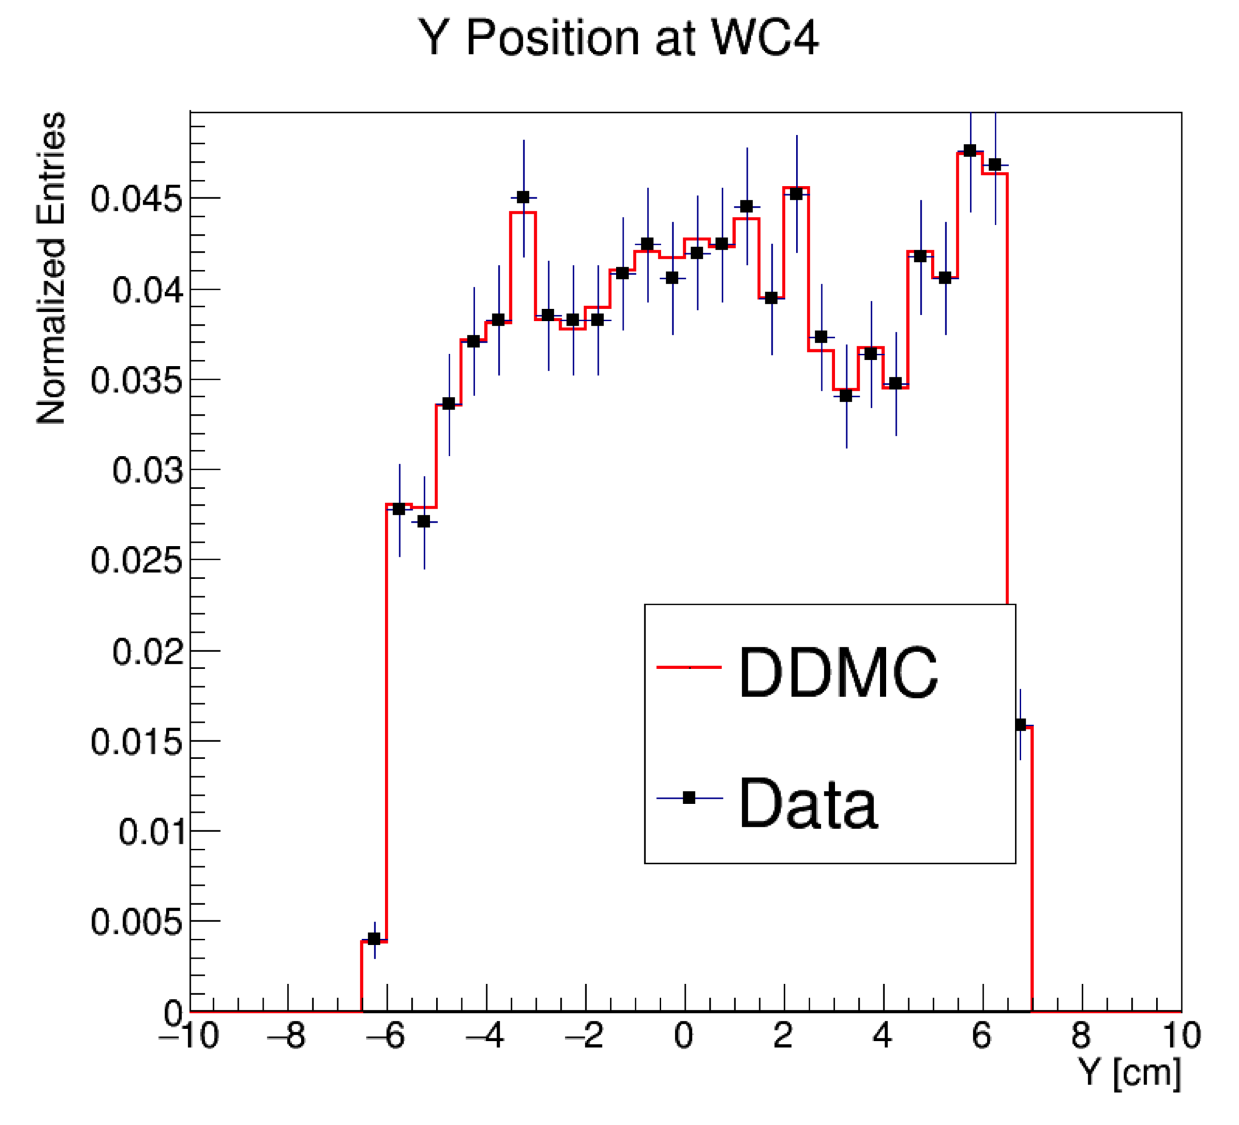
\includegraphics[width=0.48\textwidth]{Chapter-5/Images/DDMCY.png}
\caption{Comparison between generated quantities and data distributions for the 100A kaon sample: Z component of the momentum at WC4 (top left), X position at Wire Chamber 4 (top right), Y position at Wire Chamber 4 (bottom).}
\label{fig:DDMCComparison}
\end{figure}





\section{Estimate of Backgrounds in the Pion Cross Section}\label{ch:PionXSBkgSub}

We use the beamline simulation and the DDMC simulation to estimate the background in the total hadronic pion cross section. Two categories of background exists for the negative pion cross section measurement: the one related to the pion interaction in the chamber, discussed in Section \ref{ch:CaptureAndDecay} and the one related to the beamline contamination, discussed in Section \ref{ch:PionXSBkgSub2}.

\subsection{Background from Pion Capture and Decay}\label{ch:CaptureAndDecay}
Our goal is to measure the total hadronic cross section for negative pions in argon. Since pion capture can be classified as an electromagnetic process and pion decay is a week process,  capture and decay represent unwanted interactions. We present here a study of capture and decay in Monte Carlo and the solution we adopted to mitigate their occurrence in the data sample. 

For this MC study, we use a sample of  MC pions generated according to the  $-6$0A beam profile with the DDMC (see Section \ref{sec:DDMC}). It is important to notice that capture occurs predominantly at rest, while decay may occur both in flight and at rest. Thus, we can highly mitigate capture and decay at rest by removing pions which would release all their energy in the TPC and stop. This translates into a momentum selection, where we keep only events whose WC momentum is above a certain threshold. 
Figure \ref{fig:CaptureMom} shows the true momentum distribution for the primary pions\footnote{We use here the Geant4 denomination ``primary" to indicate that the pion considered does not undergo interactions modifying its energy before getting to the TPC. In fact, not every pion shot from wire chamber four will arrive to the TPC as primary,  some will decay or interact before the TPC.}  that arrive to the TPC (pink), that capture (green) or decay (blue) inside the TPC, on a linear scale (left) and on a log scale (right) vertical axis. 




In order to choose the selection value for the wire chamber momentum, it is beneficial to estimate the ratio of events which capture or decay that survive the selection in MC as a function of the momentum threshold, and compare it with the survival ratio for all the 60A events. This is done in figure \ref{fig:survRatio}. We define the survival ratio simply  as the number of events surviving the true momentum selection divided by the number of events of that category. We calculate the survival ratio separately for the three event categories explained above: total (pink), capture (green) and decay (blue).
Selecting pions with momentum greater than 420 MeV/c reduces the capture events by ~99\% while maintaining about 80\% of the 60A data sample and almost the entire 100A sample. 
Figure \ref{fig:evtRatio} shows the ratio of events which end their life in capture (green) or decay (blue) over the total number of events as a as a function of the true momentum at wire chamber four. This ratio is slightly dependent on the inelastic cross section implemented in Geant4, as we are able to register a pion capture (or decay) only if it did not interact inelastically in the TPC. We choose a momentum threshold of 420~MeV/c because the percentage of capture events drops below 1\% and the percentage of decays is never above 2\% for momenta greater than 420~MeV/c. After the momentum selection, we evaluate the contribution of capture and decay to be a negligibly small background to the cross section measurement compared to the background related to the beamline which we will address in the next section.

\begin{figure}[]
\centering
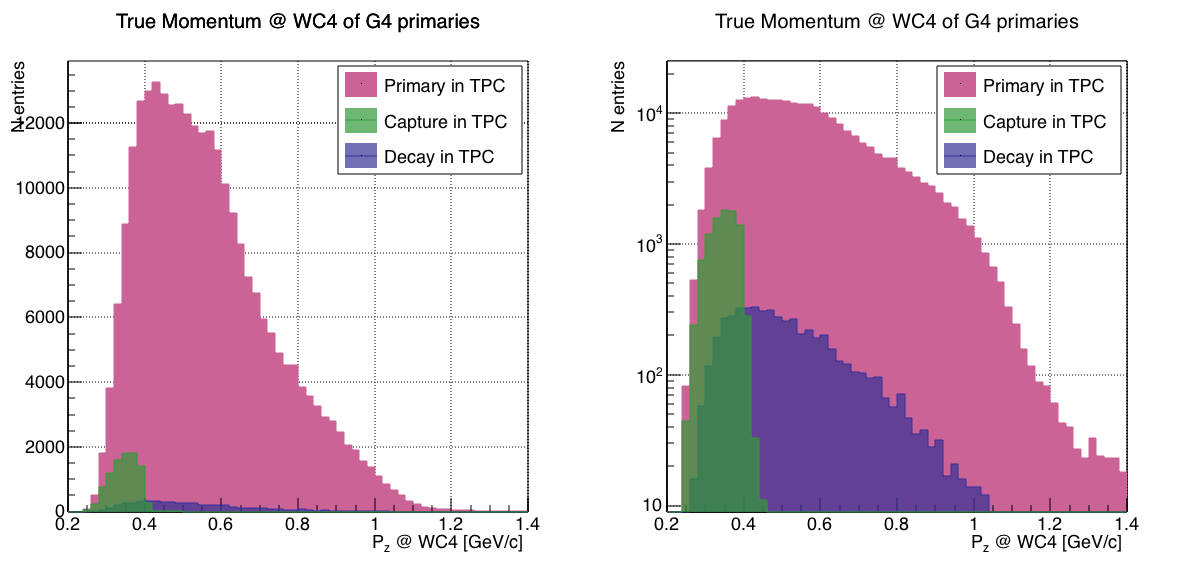
\includegraphics[width=15cm]{Chapter-7/Images/CDAsMomentumFunct.png}
\caption{True momentum distribution at wire chamber 4 for every simulated pion arriving in the TPC (pink), ending its life in capture (green) or in decay (blue) in the TPC, linear vertical axis on the left, logarithmic on the right. }
\label{fig:CaptureMom}
\end{figure}

\begin{figure}[]
\centering
\begin{minipage}[t]{0.45\textwidth}
\centering
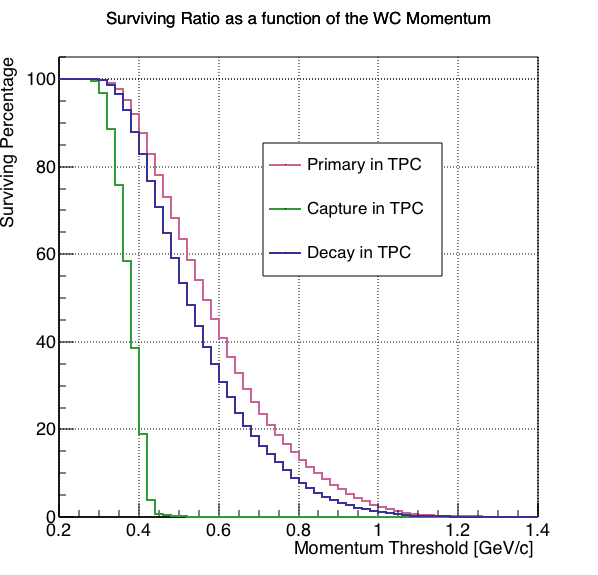
\includegraphics[width=7.5cm]{Chapter-7/Images/CDThreshold.png}
\caption{Survival ratio as a function of selection threshold on true momentum at wire chamber four for for every simulated pion arriving in the TPC (pink), capture (green) or in decay (blue).   }
\label{fig:survRatio}
\end{minipage}\hfill
\begin{minipage}[t]{0.45\textwidth}
\centering
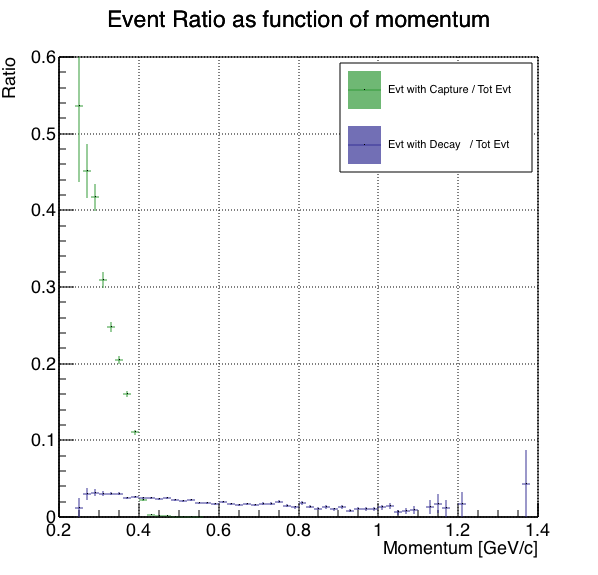
\includegraphics[width=7.5cm]{Chapter-7/Images/CDRatio.png}
\caption{Ratio between the capture (green) and decay (blue) events over the total number of events as a as a function of the true momentum at wire chamber four.}
\label{fig:evtRatio}
\end{minipage}
\end{figure}

\clearpage
%%%%%%%%%%%%%%%%%%%%%%%%%%%%%%%%%%%%%%%%%%%%%%%%%%%%%%%%%%%%
\subsection{Contributions from the Beamline Background}\label{ch:PionXSBkgSub2}
We define beamline background every TPC track matched to the WC track which is not a primary pion. Potentially, there are 4 different types of beamline background:
\begin{itemize}
\item[]1) electrons,
\item[]2) muons,
\item[]3) secondaries from pion events,
\item[]4) matched pile up events.
\end{itemize}

The first step to quantify the effect of the beamline background on the pion cross section is to estimate what percentage of events used in the cross section calculation is not a primary pion.  We start by noting that the last type of background, the ``matched pile up" events, is a negligible fraction, because of the definition of the WC2TPC match: we deem the probability of a single match with a halo particle in the absence of a beamline particle\footnote{ Events with multiple WC2TPC matches are always rejected.} negligibly small. %\textcolor{red}{SHOW VTX distribution in WC2TPC match}
As shown in Section \ref{ch:beamlineComposition}, we use G4Beamline to estimate the percentage of pions, muons and electrons at WC4, obtaining the composition shown in Table \ref{tab:beamline}. The next step is to simulate those pions, muons and electrons from WC4 to the TPC with the DDMC and evaluate their contribution to the cross section. To do so, we start by simulating the same number of electrons, muons and pions with the DDMC and we apply the same selection chain (i.e. track multiplicity rejection, WC2TPC acceptance and shower rejection) on the three samples. The number of events per particle species surviving this selection is shown on table \ref{tab:MCafterCutContaminants}. In order to reproduce the closest make up of the beam to data, we weight each event of a given particle species according to the estimated beam composition. In case of 60A runs, for example, the weights are 0.688 for pions,  0.046 for muons  and 0.266 for electrons.


It should be noted that pions may  interact hadronically in the steel or in the non-instrumented argon upstream to the TPC front face while travelling the length of between WC4 and the TPC. Or, they could decay in flight between WC4 and the TPC. One of the interaction products can leak into the TPC and be matched with the WC track, contributing to the pool of events used for the cross section calculation. We call this type of particles ``secondaries" from pion events, with a terminology inspired by Geant4.  We estimate the number of secondaries using the DDMC pion sample.  The percentage of secondaries is given by the number of matched WC2TPC tracks whose corresponding particle is not flagged as primary by Geant4.  The secondary to pion ratio is 4.9\% in the 60A sample and 4.3\% in the 100A sample.





\begin{table}[]
\centering
\begin{tabular}{| l | l | l | l | l | l | l | l | }
\hline
 &  \multicolumn{3}{|c|}{Magnet Current -60A} & \multicolumn{3}{|c|}{Magnet Current -100 A}\\

                                                  & MC $\pi^-$   & MC  $ \mu^-$ & MC  $e^-$ & MC  $\pi^-$ & MC  $\mu^-$ & MC  $e^-$  \\
\hline
&  &  &  & & &\\  
Total Initial events                     & 334500  & 334500 & 334500 &344500 &344500& 344500 \\
After Multiplicity Rejection        & 330668  & 333420 & 198065 &326576 &344208& 201380 \\
After WC2TPC Selection          & 218239  & 296333 & 91139  &230418 &300228& 98834  \\
Evts After Shower Rejection     & 208063  & 288914 &  20293 &219882 &293585& 17780  \\
&  &  &  & & &\\  
  \hline
&  &  &  & & &\\  
Selection Survival Rate           &62.3\% & 86.6\% & 6.1\% & 63.8\%& 85.5\%& 5.2\%\\
Beam Composition  @WC4      &  68.8\%   &  4.6 \%  & 26.6 \%    & 87.4 \% & 3.7 \%  & 8.9 \% \\ %
Beam Composition  @TPC FF &  88.5\%   & 8.2\%   & 3.3 \%   & 94.0\%	& 5.3\% & 0.7\%\\
                                                  &                      &                       &                   &                       &                        &\\  
\hline
\end{tabular}
\caption{MC selection flow per particle species.}
\label{tab:MCafterCutContaminants}
\end{table}


\begin{figure}[p]
\centering
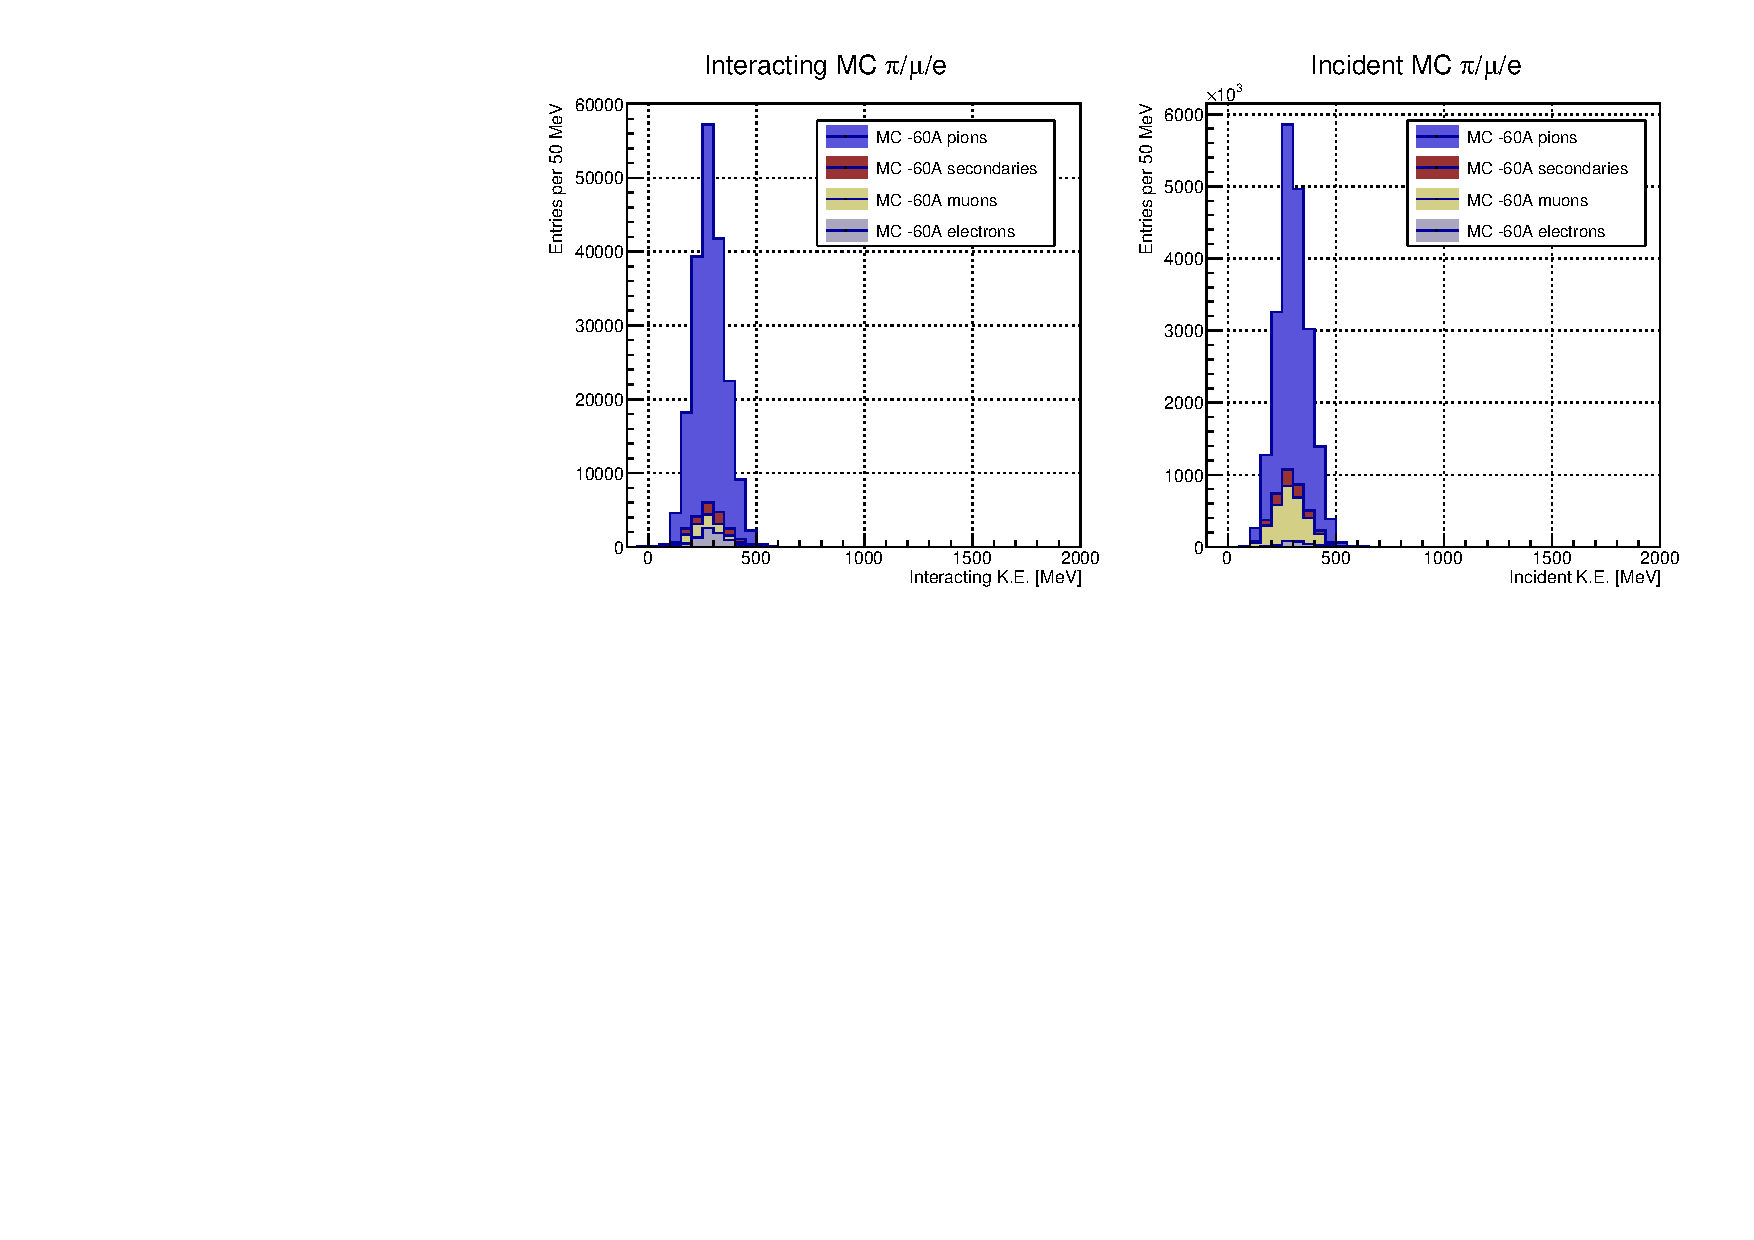
\includegraphics[width=\textwidth]{Chapter-5/Images/Background60A.pdf}
\caption{Left: staggered contributions to the interacting kinetic energy distribution for electron (grey), muons (yellow) and pion (blue) in the 60A simulation sample. Right: staggered contributions to the incident kinetic energy distribution for electron (grey), muons (yellow) and pion (blue) in the 60A simulation sample.  }
\label{fig:stag60A}
\end{figure}

We evaluate the beamline background contribution to the cross section by producing the interacting and incident histograms for the events surviving the selection, staggering the contributions for each particle species, as shown in Figure  \ref{fig:stag60A}. From those histograms, we are able to evaluate the contribution of  pions and  beamline backgrounds to each bin of the interacting and incident histograms separately and obtain the relative pion content. The relative pion content in each bin for the interacting and incident histograms represents the correction applied to data. We take here the interacting histogram as example, noting that the derivation of the correction for the incident histogram is identical. The number of entries in each bin of the interacting plot (Figure \ref{fig:stag60A} left) is  $N^{\text{TOT}}_{\text{Int}} (E_{i})$, equal to the sum of the pions and beamline backgrounds in that bin, namely

\begin{equation}
N^{\text{TOT}}_{\text{Int}} (E_{i}) =  N^\pi_{\text{Int}} (E_{i}) + \underbrace{ N^\mu_{\text{Int}} (E_{i}) + N^e_{\text{Int}} (E_{i}) + N^{Secondary}_{\text{Int}} (E_{i}) }_{B_{\text{Int}} (E_i)}.
\end{equation}
Thus, the relative pion content to each bin in MC can be calculated as follows
\begin{equation}
C^{\pi MC}_{\text{Int}} (E_{i}) =  \frac{N^{\pi MC}_{\text{Int}}}{ N^{TOT MC}_{\text{Int}} (E_{i}) } =    \frac{N^{TOT MC}_{\text{Int}} (E_{i}) - B^ {MC}_{\text{Int}} (E_i)}{ N^{TOT MC}_{\text{Int}} (E_{i})}.
\end{equation}


In order to evaluate the pion content of each bin in data, we scale the measured bin by the corresponding relative pion content found in MC, as follows
\begin{equation}
N^{\pi Reco Data}_{\text{Int}} = N^{TOT Data}_{\text{Int}} (E_{i}) - B^{Data}_{\text{Int}} (E_i)  =  C^{\pi MC}_{\text{Int}} (E_{i}) N^{TOT Data}_{\text{Int}} (E_{i}).
\end{equation}

The pion content is evaluated separately in the interacting and incident histograms. Their ratio determines a correction to the measured raw cross section. 
For example, the measured raw  cross section of a sample with enhanced muons content will tend to be lower than the raw cross section of a muon free sample. This is because most of the muons will cross the TPC without stopping, thus contributing almost exclusively to the incident histogram, forcing the pion content to be lower in the incident histogram than in the interacting; thus, the correction will tend to enhance the cross section.

\section{Estimate of Energy Loss before the TPC}\label{ch:eloss}
The beamline particles travel a path from where their  momentum is measured in the beamline until they are tracked again inside the TPC. In the LArIAT geometry, a particle leaving the WC4 will encounter the materials listed in Table \ref{tab:budget} before being registered again. The energy lost by the particle in this non-instrumented material modifies the particle's kinetic energy and directly affects the cross section measurement, as shown in equation \ref{eq:enFF}.

\begin{table}[h!]
\centering
\begin{tabular}{|l|l|l|}
\hline
Material  & density {[}g/cm$^3${]} & width {[}cm{]}    \\ \hline
Fiberglass laminate (G10)      & 1.7                             & 1.28                              \\
Liquid Argon                           & 1.4                             & 3.20                             \\
Stainless Steel                        & 7.7                            & 0.23                             \\
Titanium                                  & 4.5                            & 0.04                             \\ 
Air                                            &  1.2 $\cdot10^{-3}$  & 89.43                              \\
Plastic Scintillator                    & 1.03                          & 1.20 (+ 1.30)                 \\ \hline
\end{tabular}
\caption{LArIAT material budget from WC4 to the TPC Front Face.}
\label{tab:budget}
\end{table}


We derive an estimate of the energy loss between the beamline momentum measurement and the TPC ($E_{loss}$) from the pion and kaon DDMC samples, since this quantity is not  measurable directly on data. 
The $E_{loss}$ distribution for the 60A  and 100A pion sample is shown in figure \ref{fig:ELoss60A}, left and right respectively. The $E_{loss}$ distribution for the  whole kaon sample is shown in figure \ref{fig:ELossKaons}. A clear double peaked structure is visible, which is due to the particles either missing or hitting the HALO paddle: a schematic rendering of this occurrence is  shown in figure \ref{fig:Halo}. The kinematic at WC4 determines the trajectory of a particle and whether or not it will hit the halo paddle. In figure \ref{fig:PxVsXTrue} , we plot the true  horizontal component of the momentum $P_x$ versus the true $X$ position at WC4 for pions missing the halo paddle (left) and for pions hitting the halo paddle (right) for the -60A MC simulation runs -- analogous plots are obtained with the -100A pion simulation and with the kaon simulation. These distributions can be separated drawing a line in this position-momentum space. 
We use a logistic regression  \cite{agresti2013categorical}  as a classifier to find the best separating line, shown in both plots as the red line. We classify as ``hitting the halo paddle" all pions whose $P_x$ and $X$ are such that $$P_x +0.02* X - 0.4 < 0 $$ and as ``missing the halo  paddle" all pions whose $P_x$ and $X$ are such that $$P_x +0.02*X - 0.4 > 0, $$ where the coefficients of the line are empirically found by the logistic regression estimation. Overall, this simple method classifies in the right category (hit or miss) about 86\% of the pion events. In MC, we assign  $E_{loss} = 32 \pm 4 $~MeV for pion events classified as ``hitting the halo paddle"; we assign  $E_{loss} = 24 \pm 3 $~MeV for pion events classified as ``missing the halo paddle". We apply the same classifier on data. 

A scan of the simulated geometry showed an excess of 3 cm of uninstrumented argon compared with the surveyed detector geometry. We account for this difference by assigning in data $E_{loss} = 24 \pm 6 $~MeV for pion events classified as ``hitting the halo paddle" and  $E_{loss} = 17 \pm 6 $~MeV for pion events classified as ``missing the halo paddle", where the uncertainty is derived as the standard deviation of the double peaked distribution.

The summary of the values for used for $E_{Loss}$ for the pion sample is listed in table \ref{tab:Eloss}  with the analogous results for the study on the kaon case.

\begin{table}[b]
\centering
\begin{tabular}{|l|c|c|}  
\hline
                          &  \multicolumn{2}{c|}{E$_{loss}$ [MeV]}    \\ \hline
                          & Hitting Halo          & Missing Halo     \\ \hline
Pion  MC           &  $32 \pm 4 $         &    $24 \pm 3$     \\ \hline
Pion Data          &  $25 \pm 6$          &    $17 \pm 6 $    \\ \hline
Kaon  MC          &  $38 \pm 6 $        &     $31 \pm 5 $    \\ \hline
Kaon Data         &  $26 \pm 7 $        &     $22 \pm 7 $    \\ \hline
\end{tabular}
\caption{Energy loss for pions and kaons.}
\label{tab:Eloss}
\end{table}



%We use the separation of these two distributions to decide what the energy loss for each event on data. 
%Thus,  we assign the value for energy loss is used in the data.


\begin{figure}[hbpt]
\centering
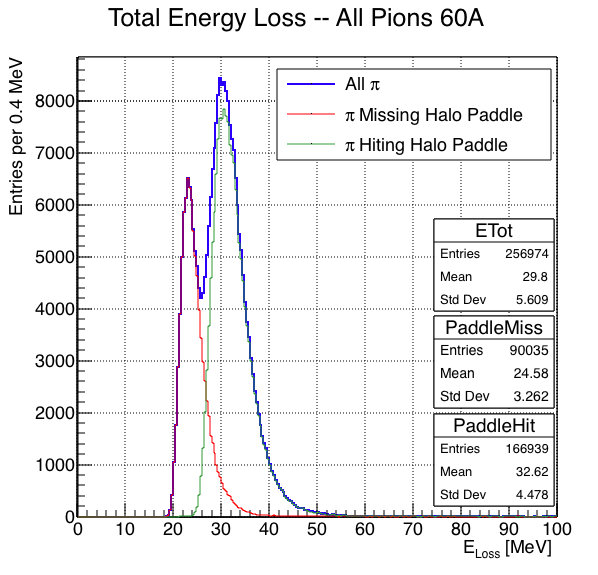
\includegraphics[width=0.45\textwidth]{Chapter-5/Images/E_loss60A.png}
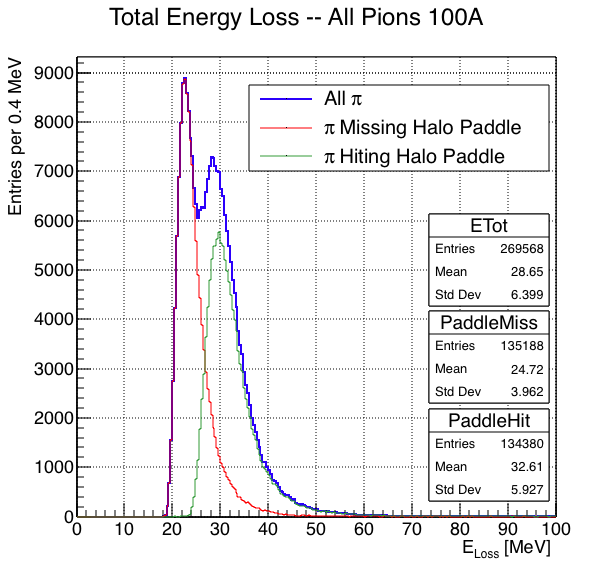
\includegraphics[width=0.45\textwidth]{Chapter-5/Images/E_loss100A.png}
\caption{True energy loss between WC4 and the TPC front face according to the MC simulation of negative pions of the 60A runs (left) and of the 100A runs (right). The distribution for the whole data sample is shown in blue, the distribution for the pions missing the halo is shown in red, and the distribution for the pions hitting the halo is shown in green.  }
\label{fig:ELoss60A}
\end{figure}

\begin{figure}[hbpt]
\centering
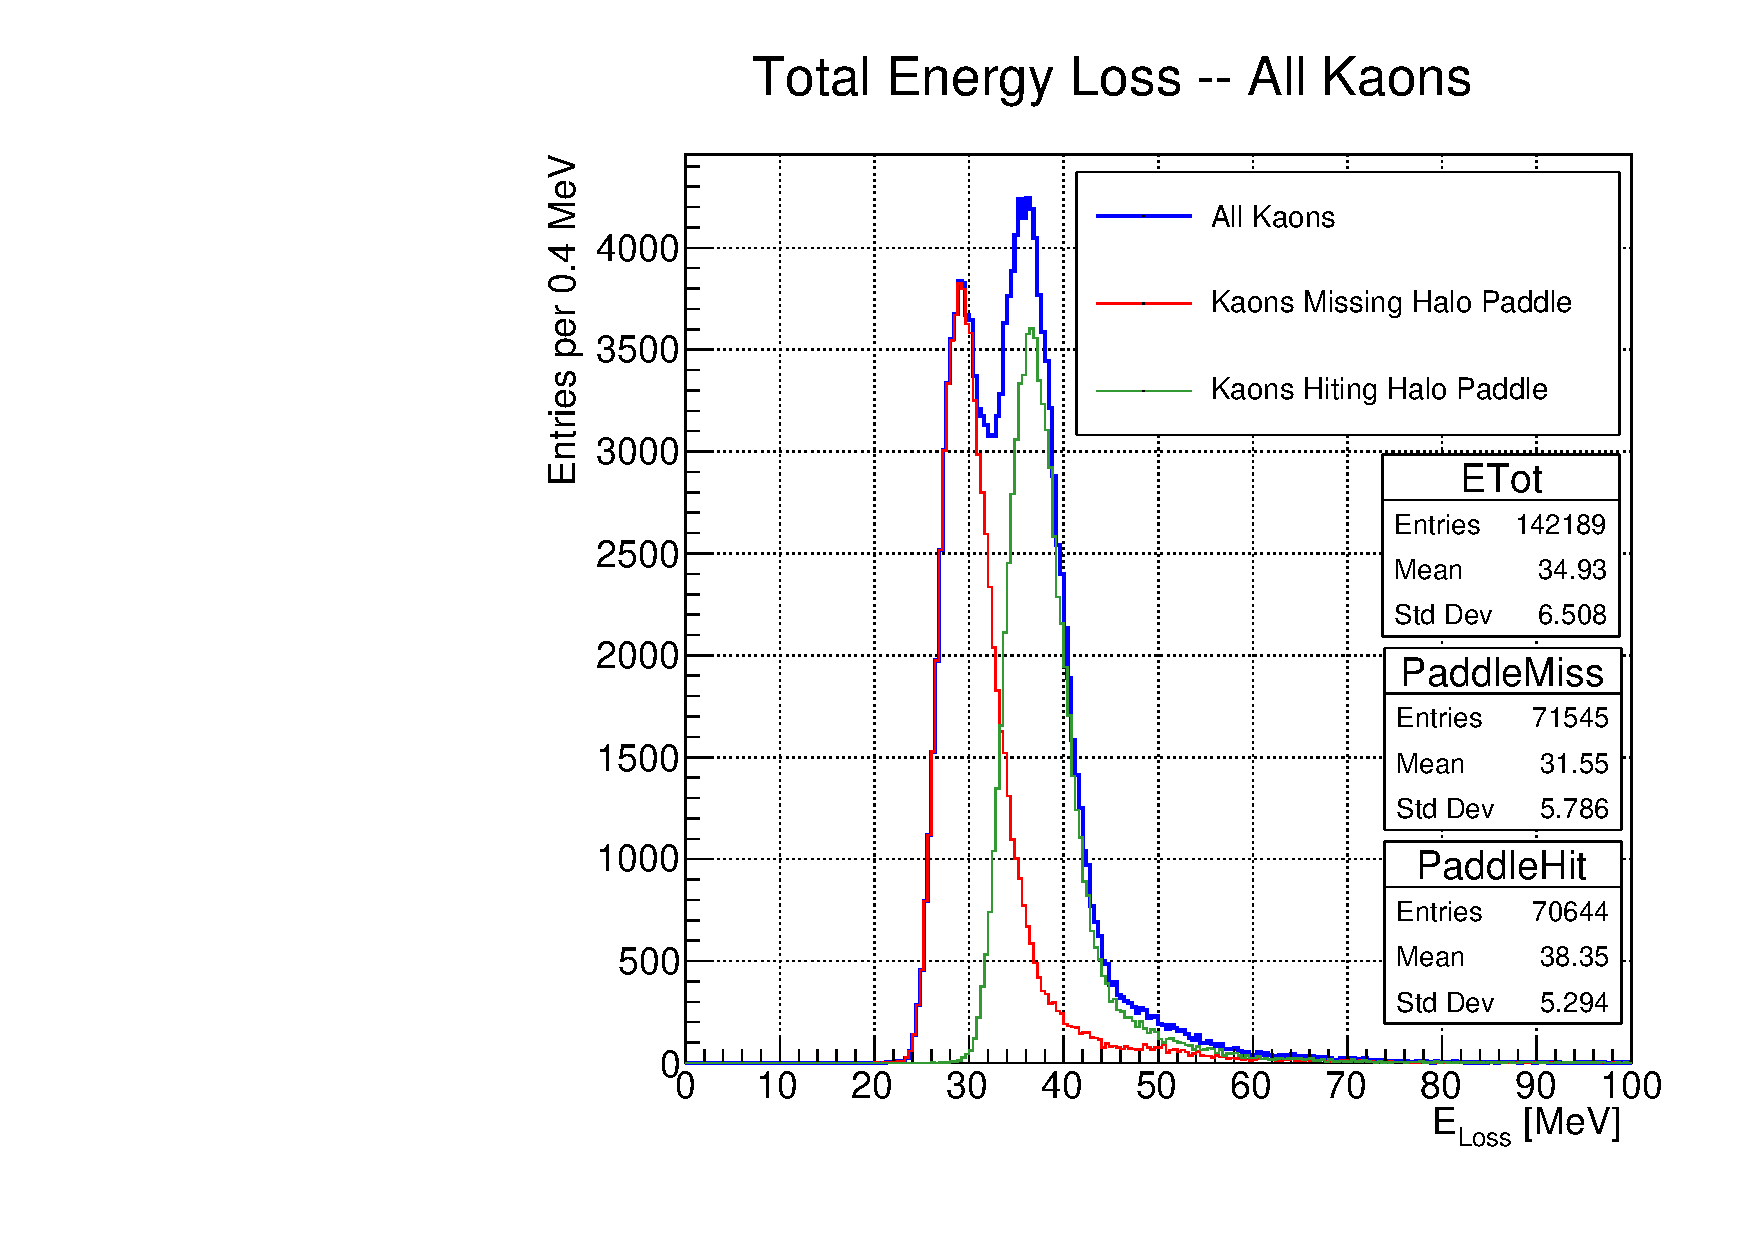
\includegraphics[width=0.45\textwidth]{Chapter-5/Images/ELossKaons.pdf}
\caption{True energy loss between WC4 and the TPC front face according to the MC simulation of positive kaons in the 60A and 100A combined sample. The distribution for the whole data sample is shown in blue, the distribution for the kaons missing the halo is shown in red, and the distribution for the kaons hitting the halo is shown in green.  }
\label{fig:ELossKaons}
\end{figure}




\begin{figure}[hbpt]
\centering
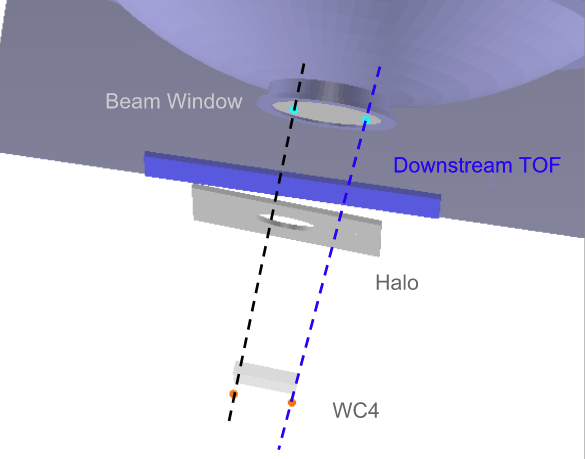
\includegraphics[scale=0.5]{Chapter-5/Images/Halo.png}
\caption{Schematic rendering of the particle path between WC4 and the TPC front face. The paddle with the hollow central circle represents the Halo paddle. We illustrate two possible trajectories: in black, a trajectory that miss the paddle and goes through the hole in the Halo, in blue a trajectory that hits the Halo paddle and goes through the scintillation material.}
\label{fig:Halo}
\end{figure}



\begin{figure}[hbpt]
\centering
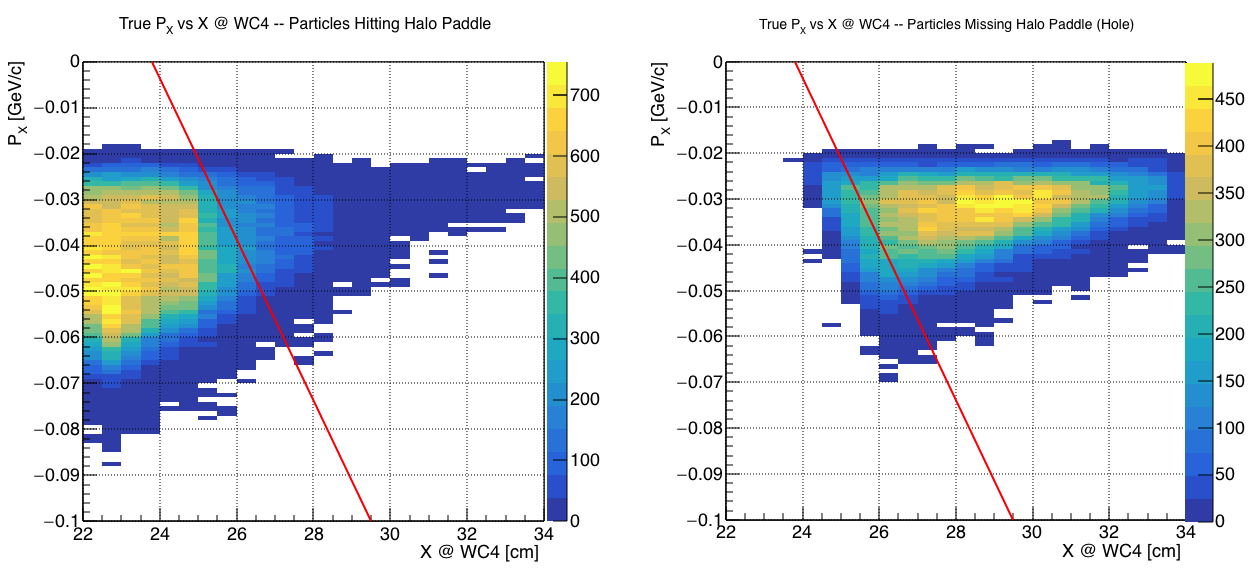
\includegraphics[width=\textwidth]{Chapter-5/Images/PXVsX60A.png}
\caption{Horizontal component of the true momentum vs the horizontal position at WC4 for MC simulated pions of the 60A runs. The plot on the left shows the distribution for pion that miss the halo paddle and the plot on the right shows the distributions for pions that hit the halo. The form of the classifier is overlaid to both plots (red line).}
\label{fig:PxVsXTrue}
\end{figure}

\section{Tracking Studies}\label{sec:TrackingStudies}
The tracking of hadrons in the TPC determines both the beamline to TPC handshake and the identification of the interaction point within the TPC. Thus, it plays a fundamental role in the cross section measurements. We performed several studies geared towards the optimization of the package for tracking in the TPC. In particular, we studied a suitable set of parameters for the WC2TPC match and we optimized the clustering algorithm to maximize the efficiency of finding the interaction point on MC. Given the technical nature of these studies, we report them in Appendix \ref{ch:AppendixTrack}. 
We report here the evaluation of  the angular resolution of the tracking algorithm in data and MC, due to its implication on the physics measurement.


\subsection{Angular Resolution}\label{sec:angleRes}
Scope of this study is to understand and compare the tracking performances and angular resolution of the TPC tracking on data and MC. 
We use the angular resolution of the tracking to determine  the value of smallest angle that we can reconstruct with a non-zero efficiency, effectively determining a selection on the angular distribution of the cross section measurement due to the tracking performance. This study is performed on the pion sample, but its results are extrapolated to the kaon case.

We start by selecting all the WC2TPC matched tracks used for the cross section analysis.  These tracks can contain from a minimum of 3 3D-space points to a maximum of 240  3D-space points.  We fit a line to all the 3D-space points associated with the track. 
For each track we calculate the average distance between each point in space and the fit line as follows 
\begin{equation} 
\bar d = \frac{\sum^N_i d_i}{N},
\end{equation} 
where $N$ is the number of 3D-space points of the track and $d_i$ is the distance of the $i$-th space point to the line fit. Several tests to compare the goodness of fit between data and MC have been considered. We decided to use $\bar d$ for its straightforward interpretation. The $\bar d$ distribution for data and MC is shown in Figure \ref{fig:Chi2AllPts} and shows a relatively good agreement between data and MC.

A visual representation of the procedure used to evaluate the angular resolution is shown in Figure \ref{fig:AngResProcedure}. 
For each track, we order the space points according to their Z position along the positive beam direction (panel a) and we split them in two sets: the first set contains all the points belonging to the first half of the track and the second set contains all the points belonging the second half of the track. We remove the last four points in the first set and the first four points in the second set, so to have a gap in the middle of the original track (panel b). We fit the first and the second set of points with two lines  (panel c). We then calculate the angle between the fit of the first and second half $\alpha$ (panel d). The angle $\alpha$ determines the spatial resolution of the tracking. The distributions for data and MC for $\alpha$ are given in Figure \ref{fig:trackingResolution}. The mean of the data and MC angular resolution are respectively 

\begin{equation}
\bar\alpha_{Data} = (5.0 \pm 4.5) \text{ deg}, 
\end{equation}

\begin{equation}
\bar\alpha_{MC} = (4.5 \pm 3.9) \text{ deg}. 
\end{equation}

Interaction angles smaller than the angle resolution are indistinguishable for the reconstruction. Therefore, we assess our ability to measure the cross section to be limited to interaction angles greater than 5.0 deg. More accurate studies of the angular resolution as a function of the kinetic energy and track length, albeit interesting, are left for an improvement of the analysis. 

It is beneficial to take a moment to describe the definition of interaction angle. In case of elastic scattering, the definition is straightforward: the interaction angle is the angle between the incoming and outgoing pion, i.e.

\begin{equation}  
\theta = \cos^{-1} \Big(\frac{\vec p _{\text{incoming}}  \cdot\vec p _{\text{outgoing}}}{|\vec p _{\text{incoming}}|  |\vec p _{\text{outgoing}}| }\Big).
\end{equation}   
In case of inelastic scattering,  the presence of several topologies requires a more complex definition, as shown in figure \ref{fig:scatterPic}.  We define the scattering angle as the biggest of the angles between the incoming pion and the visible daughters, where the visible daughters are charged particles that travel more than 0.47 cm in the detector (see panel a); in case all the daughters are invisible, the angle is assigned to be 90 deg (see panel b). We chose this working definition of scattering angle for inelastic scattering keeping in mind how our tracking reconstruction works: the tracking will stop correctly in case of all the daughters are not visible in the detector and it is likely to stop correctly if multiple daughters form an interaction vertex. The only ``dangerous" case is the production of one charged daughter plus neutrals, which we can study with this working definition of scattering angle (see panel c).


We can see the effects of the angular resolution on the cross section by plotting the true Geant4 cross section for interaction angles greater than a minimum interaction angle. Figure \ref{fig:trueWithAngles} shows the  true Geant4 cross section  for interaction angles greater than 0 deg (green), 4.5 deg (red), 5.0 deg  (blue) and 9.0 deg (yellow). 
A small $0.5 \text{ deg}$ systematic shift between the mean of the data and MC angular resolution is present.%, which we account for in the context of the MC efficiency correction to the cross section, as presented in \ref{sec:angSys}.


\begin{figure}[ht]
\begin{minipage}[t]{0.45\linewidth}
\centering
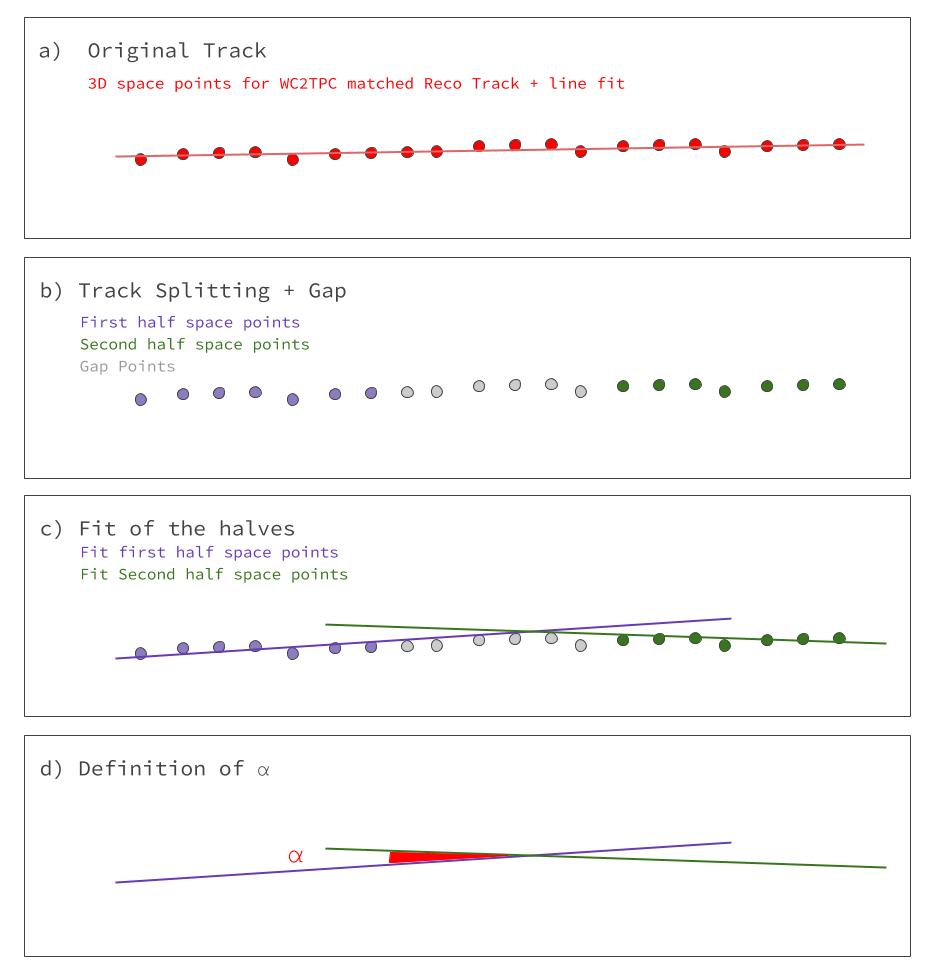
\includegraphics[width=\textwidth]{Chapter-5/Images/TrackingProcedure.png}
\caption{A visual representation of the procedure used to evaluate the angular resolution.}
\label{fig:AngResProcedure}
\end{minipage}
\hspace{0.5cm}
\begin{minipage}[t]{0.45\linewidth}
\centering
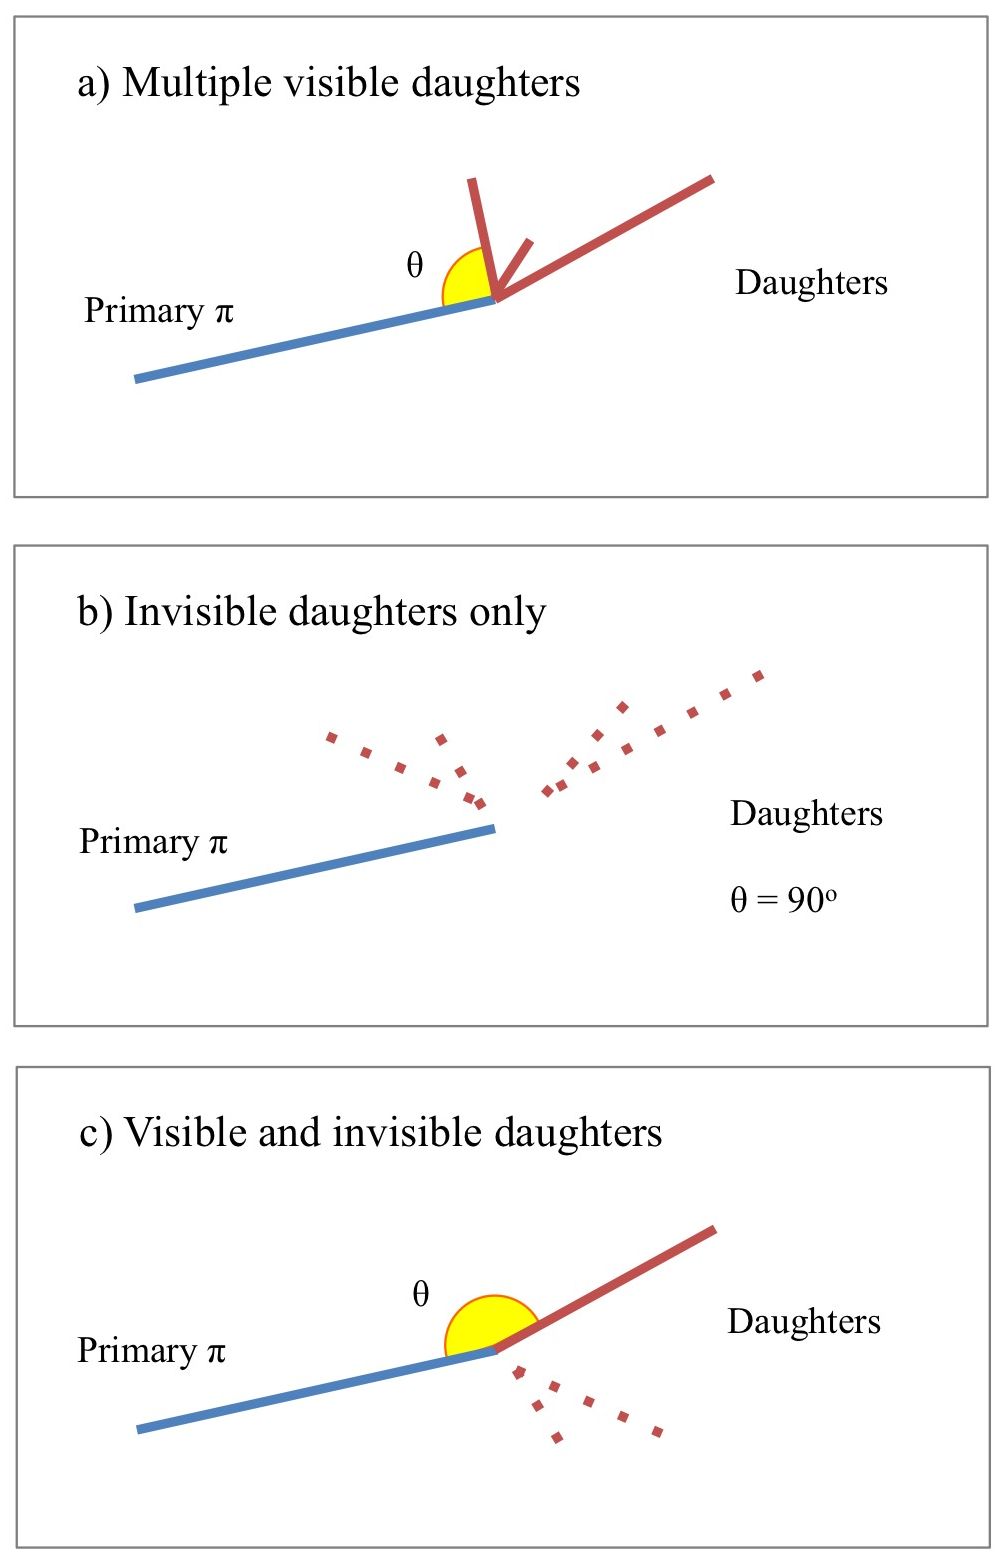
\includegraphics[width=\textwidth]{Chapter-5/Images/Daughters.png}
\caption{A visual representation of the scattering angle definition in case of inelastic scattering.}
\label{fig:scatterPic}
\end{minipage}
\end{figure}


\begin{figure}[ht]
\begin{minipage}[t]{0.45\linewidth}
\centering
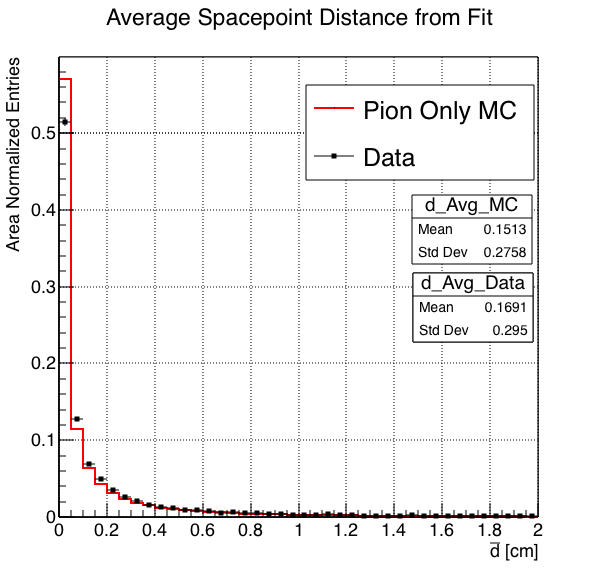
\includegraphics[width=\textwidth]{Chapter-5/Images/cDAvg.png}
\caption[]{Distributions of the average distance between each 3D point in space and the fit line,  $\bar d$ for the data used in the pion cross section analysis and the pion only DDMC. The distributions are area normalized. } \label{fig:Chi2AllPts}
\end{minipage}
\hspace{0.5cm}
\begin{minipage}[t]{0.45\linewidth}
\centering
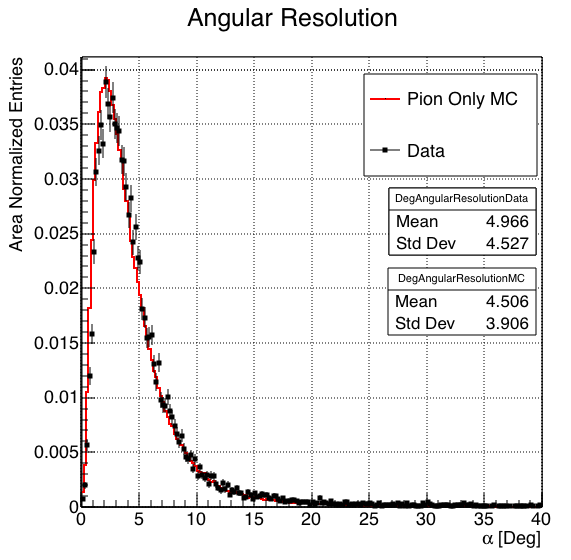
\includegraphics[width=\textwidth]{Chapter-5/Images/cTrackingDeg.png}
\caption[]{Distributions of angular resolution $\alpha$ for data used in the pion cross section analysis and pion only DDMC. The distributions are area normalized. } \label{fig:trackingResolution}
\end{minipage}
\end{figure}



	
	

\begin{figure}[ht]
\begin{minipage}[t]{0.45\linewidth}
\centering
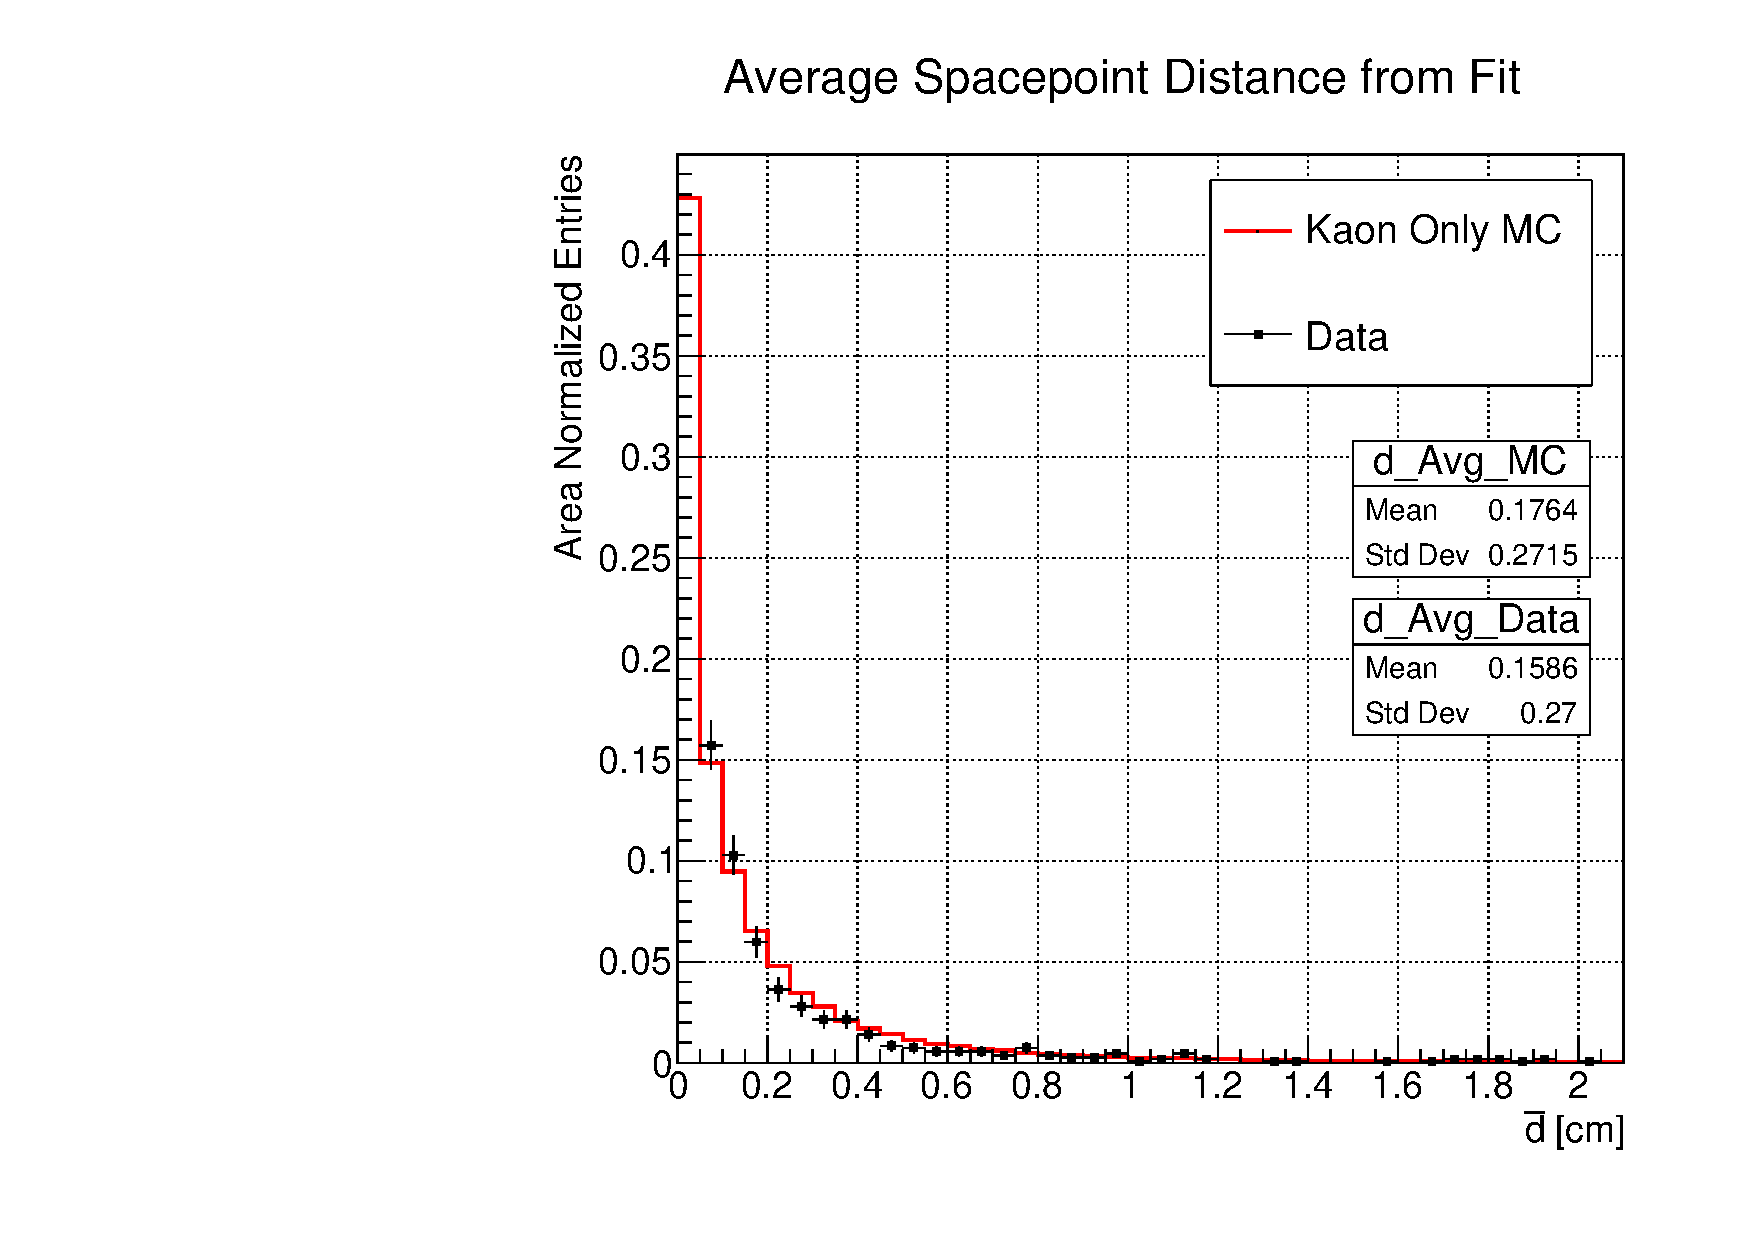
\includegraphics[width=\textwidth]{Chapter-5/Images/DavgKaons.pdf}
\caption[]{Distributions of the average distance between each 3D point in space and the fit line,  $\bar d$ for the data used in the kaon cross section analysis and the kaon only DDMC. The distributions are area normalized. } \label{fig:Chi2AllPts}
\end{minipage}
\hspace{0.5cm}
\begin{minipage}[t]{0.45\linewidth}
\centering
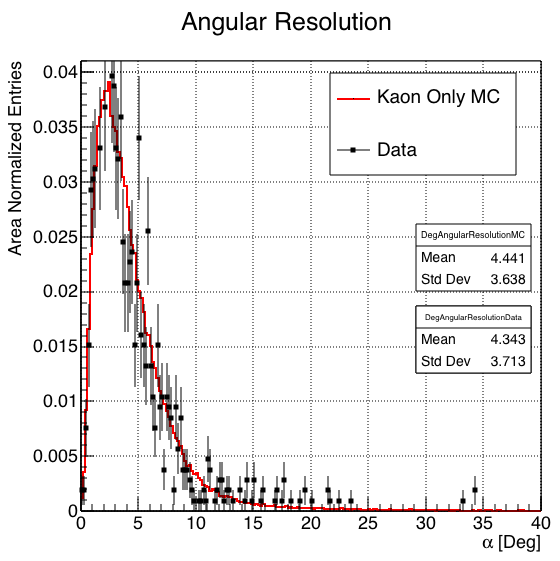
\includegraphics[width=\textwidth]{Chapter-5/Images/KaonAngRes.png}
\caption[]{Distributions of angular resolution $\alpha$ for data used in the kaon cross section analysis and kaon only DDMC. The distributions are area normalized. } \label{fig:trackingResolutionK}
\end{minipage}
\end{figure}





\begin{figure}[p]
\centering
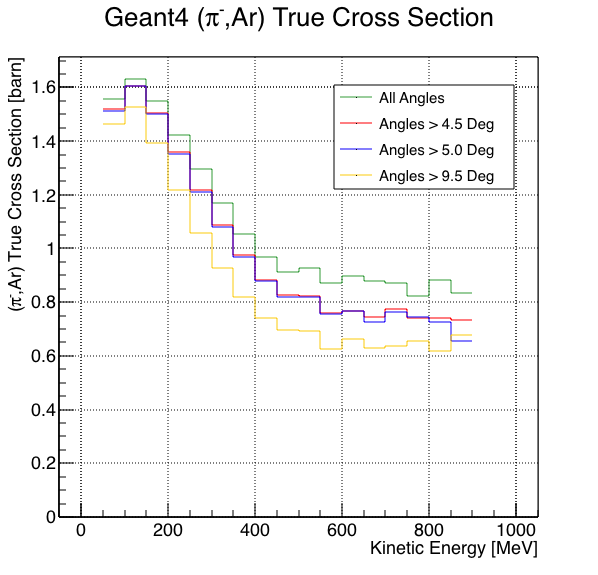
\includegraphics[width=0.48\textwidth]{Chapter-5/Images/cTrueXSAngle.png}
\caption{ True ($\pi^-, Ar$) cross section for interaction angles greater than 0 deg (green), 4.5 deg (red), 5.0 deg  (blue) and 9.0 deg (yellow). }
\label{fig:trueWithAngles}
\end{figure}



\clearpage
%%%%%%%%%%%%%%%%%%%%%%%%%%%%%%%%%%%%%%%%%%%%%%%%%%%%%%%%%%%%%%
%%%%%%%%%%%%%%%%%%%%%%%%%%%%%%%%%%%%%%%%%%%%%%%%%%%%%%%%%%%%%%
%%%%%%%%%%%%%%%%%%%%%%%%%%%%%%%%%%%%%%%%%%%%%%%%%%%%%%%%%%%%%%

\section{Calorimetry Studies}\label{ch:energyCal} 
The ability to measure the kinetic energy of hadrons in the TPC is fundamental for the cross section analyses. 
Thus, we describe first how we calibrate the TPC calorimetric response (Section \ref{ch:energyCalibration}) and how we measure the kinetic energy of the hadrons in the TPC (Section \ref{ch:kinEn}).




\subsection{Kinetic Energy Measurement}\label{ch:kinEn}
The measured kinetic energy of a hadron candidate at each argon slab determines which bins of the interacting and incident histograms a selected event is going to fill. In this section, we define the measurement on the kinetic energy and  determine the related uncertainty. We will propagate this uncertainty into the cross section measurement, as discussed in Section \ref{ch:SysUncertaintyXSRaw} for the pion cross section and in Section \ref{ch:KaonXSRawUnc} for the kaon cross section.

The kinetic energy of a hadron at the $j^{\text{th}}$ slice of argon in the TPC is given by

\begin{equation}
KE_{j} = \sqrt{p_{Beam}^2 + m_{Beam}^2} - m_{Beam}^2 - E_{Loss} - E_{\text{FF-j}},
\end{equation}

where $p_{Beam}$ is the momentum measured by the beamline detectors,  $m_{Beam}$ is the mass of the hadron as reported in the PDG,  $E_{Loss}$  is the energy loss between the beamline and the TPC, and $ E_{\text{FF-j}}$ is the energy that the hadron deposited from the TPC front face until the $j^{\text{th}}$ slice.
The uncertainty on $KE_{j}$ is then given by 
\begin{equation}
\delta KE_{j} = \sqrt{\delta p_{Beam}^2 + \delta E_{Loss}^2 +  \delta  E_{\text{dep FF-j}}^2},
\end{equation}

where we have dropped the uncertainty on the mass, since it is orders of magnitude smaller than the other uncertainties.
We assume the relative uncertainty on $p_{Beam}$ to be 2\%, and the uncertainty on the energy loss upstream to be 7~MeV, as calculated in Section \ref{ch:eloss}. We describe the estimate of the uncertainty on $E_{\text{FF-j}}$ in the rest of this section.

The energy deposited by the hadron from the TPC front face until the $j^{\text{th}}$ slice is the sum of the measured energy deposited in each previous slabs $E_{i}$, i.e.
\begin{equation}
E_{\text{FF-j}} = \sum_{i<j} E_{i}, 
\end{equation}
where $E_{i}$ is measured in each slab as  the product of the stopping power,  $dE/dX_{i}$,  and the track pitch, $Pitch_i$, for that point. 
If we assume conservatively that the measurements of $E_{i}$ are not independent from one another, the uncertainty on $E_{\text{FF-j}}$ becomes
\begin{equation}
\delta E_{\text{FF-j}} = (j-1) \delta E_{i}, 
\end{equation}
where $\delta E_{i}$ is the uncertainty on the energy loss in one slab of argon.

The left side of Figure \ref{fig:EnergyDeposited} shows the distribution of the energy deposited in each slab of argon, for the 60A negative pion dataset in black and for the pion only MC in blue. The analogous plot for the -100A negative pion data set  is show on the right side of Figure \ref{fig:EnergyDeposited}.  The distributions are fitted with a landau displayed in red for data and in teal for MC.
The uncertainty on $E_{i}$ is given by the width of the Landau fit to the data. A small systematic uncertainty  is given by a 1.0\% difference between the most probable value of the landau fits in data and MC.

\begin{figure}[htb]
\centering
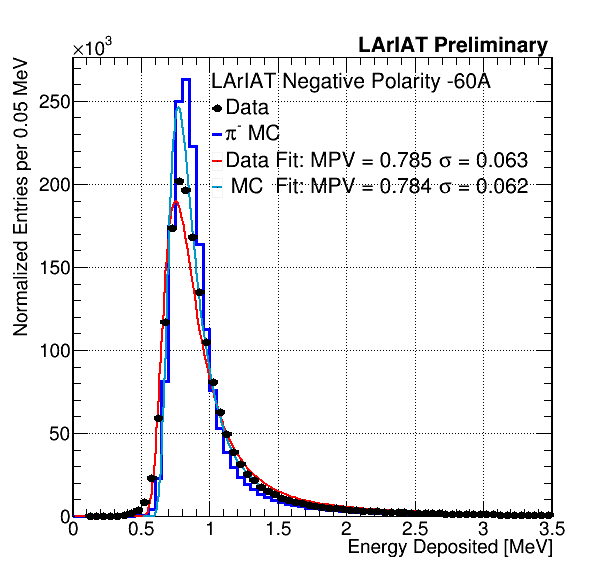
\includegraphics[width=0.48\textwidth]{Chapter-5/Images/DepEnergy_Fit_v4.png}
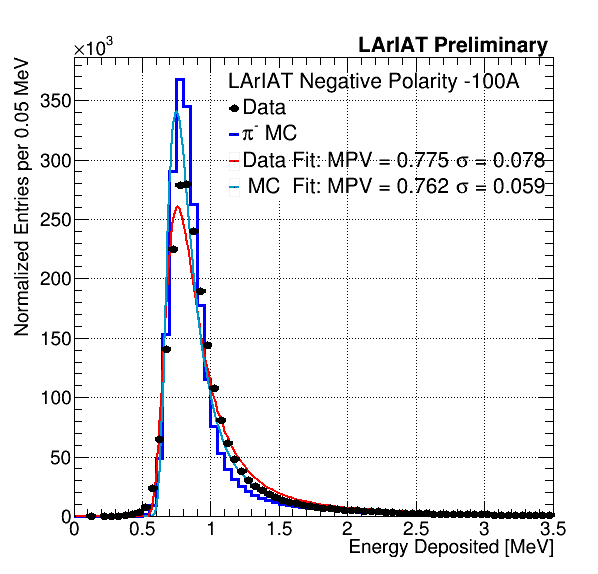
\includegraphics[width=0.48\textwidth]{Chapter-5/Images/DepEnergy_Fit_v4100A.png}
\caption[]{ Energy deposited  $E_{i}$ in a single slab of argon for the pion -60A runs (left) and -100A runs (right).  The data is shown in black, the MC in blue. The distributions are fitted with a landau displayed in red for data and in teal for MC. } \label{fig:EnergyDeposited}
\end{figure}


\begin{comment}

Figure \ref{fig:EnergyDepositedStacked} shows the stacked version of the Energy Deposited plots with the backgrounds stacked. The backgrounds are given in the ratio of 68.8\% pion, 4.6\% muon, and 26.6\% electron. Once they are taken in these ratios, the sum of the MC is normalized to the sum of the data.

\begin{figure}[htb]
\centering
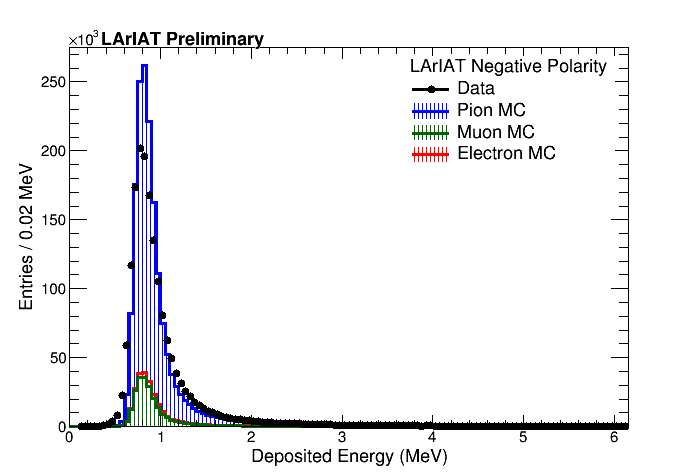
\includegraphics[width=0.48\textwidth]{Chapter-5/Images/DepEnergy_Stacked_v1.png}
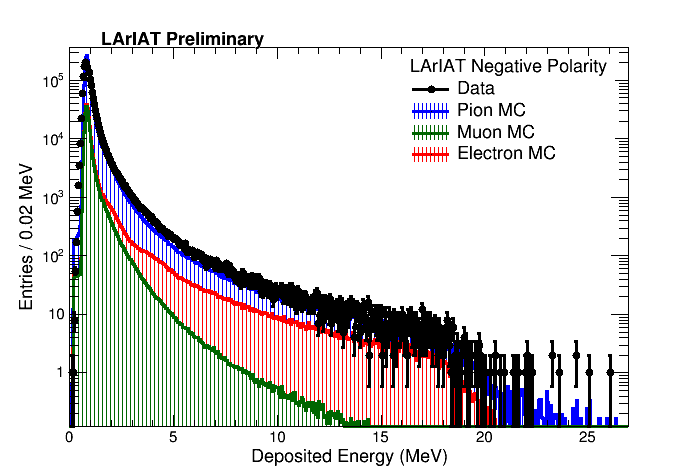
\includegraphics[width=0.48\textwidth]{Chapter-5/Images/DepEnergy_Stacked_v3.png}
\caption[]{ Energy Deposited with all the MC and 60A data.  } \label{fig:EnergyDepositedStacked}
\end{figure}

The energy at the interacting point is given by
\begin{equation}
KE_{Interaction} = \sqrt{P_{WCtrk}^2 + m_{\pi}^2} - E_{Loss} - (\Sigma dE/dX_{i} \times Pitch)
\end{equation}

and has the exact same uncertainty as the incident kinetic energy plot. Thus these estimates can be applied to getting the uncertainty on the energy of the reconstructed cross-section.




%%%%%%%%%%%%%%%%%%%%%%%%%%%%%%%%%%%%%%%%%%%%%%%
\subsection{dE/dX}
%%%%%%%%%%%%%%%%%%%%%%%%%%%%%%%%%%%%%%%%%%%%%%%
Figure \ref{fig:dEdXLinearScale} shows the output of the fit of the Pion MC and the 60 Amp data. The MC is normalized to the data and both are fit to a Landau function. \footnote{The entries at dE/dX = 0 come from an uninitialized variable and can/should be taken out of these plots}

\begin{figure}[htb]
\centering
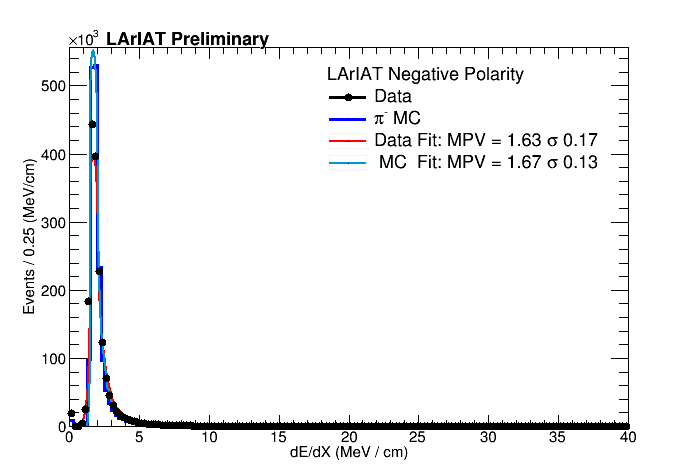
\includegraphics[width=0.48\textwidth]{Chapter-5/Images/dEdX_Fit_v1.png}
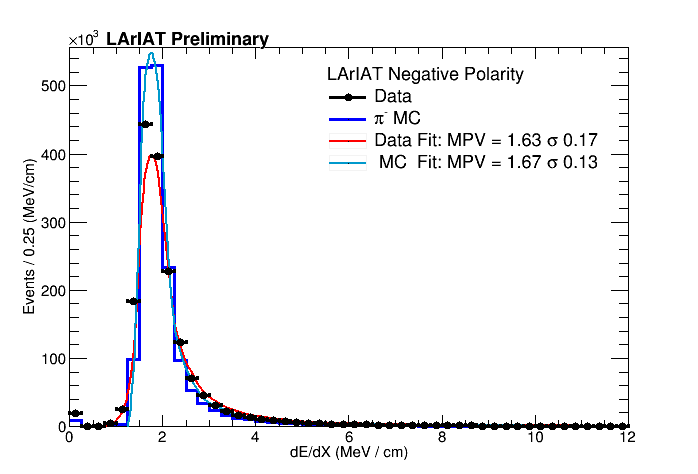
\includegraphics[width=0.48\textwidth]{Chapter-5/Images/dEdX_Fit_v4.png}
\caption[]{ dE/dX for 60Amp data and data driven pion MC, both fit with a Landau  } \label{fig:dEdXLinearScale}
\end{figure}

The difference between the two MPV's, is 2.4\% between the data and the MC.

Figure \ref{fig:dEdXLinearStacked} shows the stacked version of the dE/dX with the backgrounds stacked. The backgrounds are given in the ratio of 68.8\% pion, 4.6\% muon, and 26.6\% electron. Once they are taken in these ratios, the sum of the MC is normalized to the sum of the data.

\begin{figure}[htb]
\centering
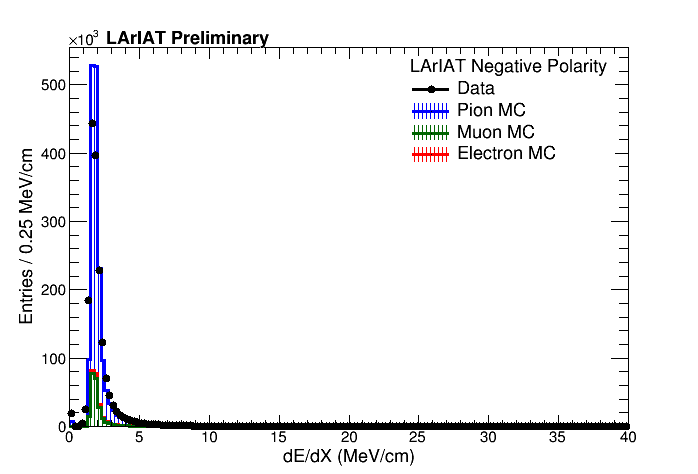
\includegraphics[width=0.48\textwidth]{Chapter-5/Images/dEdX_stacked_v1.png}
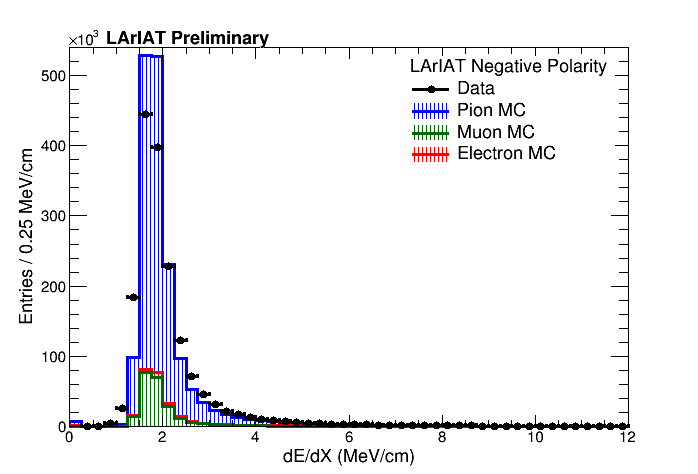
\includegraphics[width=0.48\textwidth]{Chapter-5/Images/dEdX_stacked_v4.png}
\caption[]{ Stacked versions of the dE/dX with the data and electron/muon/pion MC.  } \label{fig:dEdXLinearStacked}
\end{figure}

For completeness, the log scale versions of are shown in Figure \ref{fig:dEdXLogScale}.

\begin{figure}[htb]
\centering
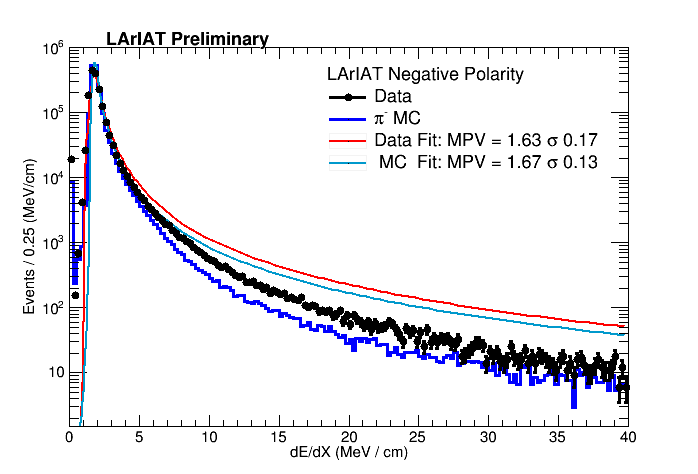
\includegraphics[width=0.48\textwidth]{Chapter-5/Images/dEdX_Fit_v2.png}
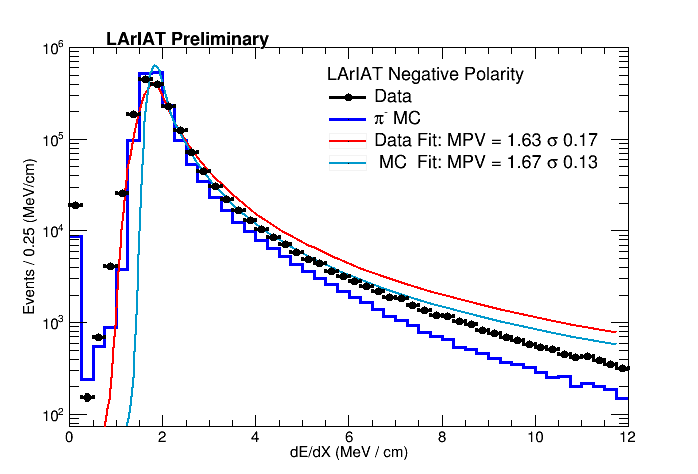
\includegraphics[width=0.48\textwidth]{Chapter-5/Images/dEdX_Fit_v3.png}
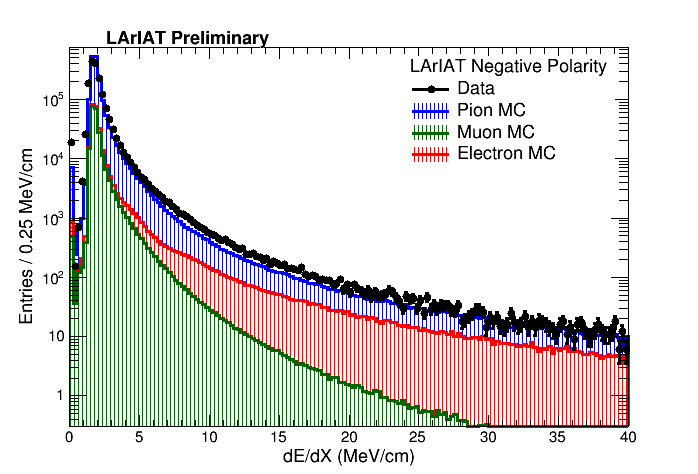
\includegraphics[width=0.48\textwidth]{Chapter-5/Images/dEdX_stacked_v2.png}
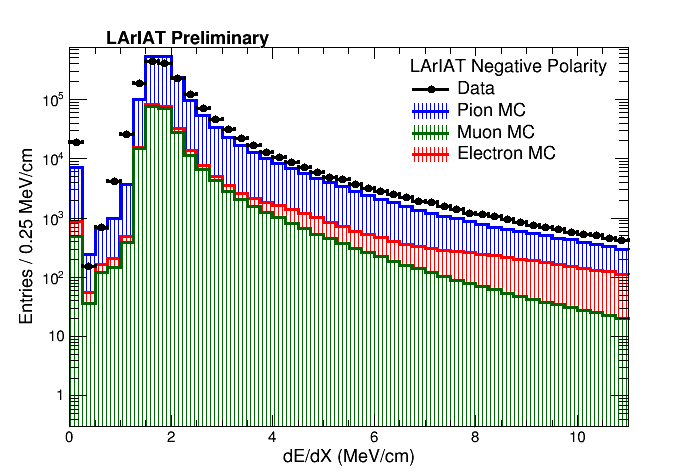
\includegraphics[width=0.48\textwidth]{Chapter-5/Images/dEdX_stacked_v3.png}
\caption[]{ dE/dX for 60Amp data and MC shown in log scale  } \label{fig:dEdXLogScale}
\end{figure}



%%%%%%%%%%%%%%%%%%%%%%%%%%%%%%%%%%%%%%%%%%%%%%%
\subsection{Energy Deposited}\label{sec:Energy}
%%%%%%%%%%%%%%%%%%%%%%%%%%%%%%%%%%%%%%%%%%%%%%%




\end{comment}




